% Bakalársky projekt 2016/2017
% Matúš Cuper

%-------------------------------------------------------------------------------
%   PACKAGES AND DOCUMENT CONFIGURATION
%-------------------------------------------------------------------------------

\documentclass[a4paper,slovak,12pt,appendix]{article}

% \usepackage{float}
\usepackage[slovak]{babel}                                                      % title in Slovak
\usepackage[utf8]{inputenc}                                                     % supported special Slovak characters
\usepackage[T1]{fontenc}                                                        % supported word wrapping on the end of line on speciacl Slovak characters
% \usepackage{url}
\usepackage{times}																															% Times New Roman
\usepackage[unicode]{hyperref}																									% enable hyper references in table of content
%\usepackage{indentfirst}                                                        % indent first line after section, but carefully, indent everything and everywhere
\usepackage{amsmath}                                                            % for fractions
\usepackage{amssymb}                                                            % for real numbers sign
\usepackage{algorithm, algpseudocode}                                           % for pseudocode writting
\usepackage{graphicx}                                                           % enable figures
\usepackage{threeparttable}                                                     % enable table with footnotes
\usepackage{url}                                                                % enable url in references chapter
\usepackage{listings}                                                           % enable source code syntax highlighting
\usepackage{courier}																														% enable monospace in listings
\usepackage{dirtree}                                                            % enable directory tree
\usepackage{caption}																														% enable caption for source under caption
\usepackage[a4paper, centering,
											left=35mm, top=25mm, right=20mm, bottom=25mm]{geometry}		% set page margins

\newcommand{\source}[1]{\caption*{\footnotesize Zdroj: {#1}} }

\lstset{
    basicstyle=\ttfamily,
		breaklines=true,
    postbreak=\raisebox{0ex}[0ex][0ex]{\ensuremath{\color{red}\hookrightarrow\space}}
}

\graphicspath{ {images/} }                                                      % set path for figures

\hypersetup{																																		% with default colours for links
    colorlinks,
		pageanchor=false,
    citecolor=black,
    filecolor=black,
    linkcolor=black,
    urlcolor=black
}

%-------------------------------------------------------------------------------
%   TITLE PAGES
%-------------------------------------------------------------------------------

\begin{document}
\begin{titlepage}
	\centering
	{\Large Slovenská technická univerzita v Bratislave \par}
	{\Large Fakulta informatiky a informačných technológií \par}
  \vspace{0.5cm}
  {\normalsize Evidenčné číslo: FIIT-5212-73688 \par}
	\vspace{7cm}
  {\large Matúš Cuper \par}
  \vspace{0.5cm}
	{\LARGE Optimalizácia konfiguračných parametrov predikčných metód \par}
	\vspace{0.5cm}
	{\large Bakalárska práca \par}
	\vspace{7cm}
  \flushleft
	{\large Vedúci práce: Ing. Marek Lóderer \par}
  \vspace{0.5cm}
  {\large máj 2017 \par}
	\vfill
\end{titlepage}

\begin{titlepage}
	\centering
  {\Large Slovenská technická univerzita v Bratislave \par}
	{\Large Fakulta informatiky a informačných technológií \par}
  \vspace{0.5cm}
  {\normalsize Evidenčné číslo: FIIT-5212-73688 \par}
	\vspace{7cm}
  {\large Matúš Cuper \par}
  \vspace{0.5cm}
	{\LARGE Optimalizácia konfiguračných parametrov predikčných metód \par}
	\vspace{0.5cm}
	{\large Bakalárska práca \\}
	\vspace{7cm}
  \flushleft
  {\normalsize Študijný program: Informatika \par}
	{\normalsize Študijný odbor: 9.2.1 Informatika \par}
	{\normalsize Miesto vypracovania: Ústav informatiky a softvérového inžinierstva, FIIT STU Bratislave \par}
	{\normalsize Vedúci práce: Ing. Marek Lóderer \par}
  \vspace{0.5cm}
  {\normalsize máj 2017 \par}
\end{titlepage}

%-------------------------------------------------------------------------------
%   ANOTATION
%-------------------------------------------------------------------------------

% \newpage\null\thispagestyle{empty}\newpage

\begin{titlepage}
\begin{center}
  {\small Slovenská technická univerzita v Bratislave \par}
  {\small \textbf{FAKULTA INFORMATIKY A INFORMAČNÝCH TECHNOLÓGIÍ}}
  \rule{\textwidth}{1pt}

  \vspace*{1.5cm}
  \begin{Large}
    \textbf{Anotácia} \par
  \end{Large}
\end{center}
{Slovenská technická univerzita v Bratislave \par}
{FAKULTA INFORMATIKY A INFORMAČNÝCH TECHNOLÓGIÍ \par}
{Študijný program: Informatika \par}
{Autor: Matúš Cuper \par}
{Bakalárska práca: Optimalizácia konfiguračných parametrov predikčných metód \par}
{Vedúci práce: Ing. Marek Lóderer \par}
{máj 2017 \\} \\
V práci sme sa zamerali na problémy vznikajúce pri predikcii časových radov.
V súčasnosti existuje veľké množstvo metód, ktoré nám zabezpečujú predpoveď
sledovanej veličiny s prijateľne malou odchýlkou na krátke obdobie v blízkej
budúcnosti. Cieľom bakalárskej práce bolo vytvoriť systém, ktorý používateľovi
poskytne jednoduché rozhranie pre porovnanie jednotlivých predikčných
algoritmov nad množinou dát, ktorú si sám zvolí. Hľadanie ich optimálneho
nastavenia sa vykonáva pomocou optimalizačných algoritmov založených na
správaní sa živočíchov v prírode.

V práci sme analyzovali a opísali množinu predikčných a optimalizačných
algoritmov. Navrhli sme systém na hľadanie optimálnych parametrov predikčných
metód, čím sme výrazne ovplyvnili ich presnosť. Systém bol implementovaný
v programovacom jazyku R a na vytvorenie používateľského rozhrania bola použitá
knižnica Shiny. Optimalizácie sme vykonávali nad dátovými množinami v doméne
energetiky. Výsledný systém umožňuje používateľovi využívať silu predikčných
algoritmov a nájsť ich optimálne parametre pre zabezpečenie čo najpresnejšej
predikcie.
\end{titlepage}

\begin{titlepage}
\begin{center}
  {\small Slovak University of Technology Bratislava \par}
  {\small \textbf{FACULTY OF INFORMATICS AND INFORMATION TECHNOLOGIES}}
  \rule{\textwidth}{1pt}

  \vspace*{1.5cm}
  \begin{Large}
    \textbf{Annotation} \par
  \end{Large}
\end{center}
{Slovak University of Technology Bratislava \par}
{FACULTY OF INFORMATICS AND INFORMATION TECHNOLOGIES \par}
{Degree Course: Computer Science \par}
{Author: Matúš Cuper \par}
{Bachelor thesis: Optimizing configuration parameters of prediction methods \par}
{Supervisor: Ing. Marek Lóderer \par}
{May 2017 \\} \\
In the thesis we focused on problems, which appear in time series prediction.
In present there are many methods, which predict observed value with acceptable
small deviation for short time period in near future. The aim of bachelor
thesis was creating system, which provides simple user interface to compare
chosen prediction algorithms on dataset, which is chosen by user. Looking for
their optimal setup is made by optimization algorithm based on nature-inspired
behavior.

In the thesis we analyzed and described set of prediction and optimization
algorithms. We designed system for searching optimal parameters of prediction
methods, which influence their accuracy significantly. System was implemented
in programming language R and for creating user interface was used library
Shiny. Optimization was provided on dataset in energetics domain. The final
system provides to user to use force of prediction algorithms and find out
their optimal parameters for the most accurate prediction.
\end{titlepage}

%-------------------------------------------------------------------------------
%   Declaration
%-------------------------------------------------------------------------------

\begin{titlepage}
\vspace*{15cm}
\begin{large}
  \noindent \textbf{ČESTNÉ PREHLÁSENIE} \par
\end{large}
\vspace*{0.5cm}
\noindent
Čestne prehlasujem, že bakalársku prácu som vypracoval samostatne pod vedením
vedúceho bakalárskej práce a s použitím odbornej literatúry, ktorá je uvedená
v zozname použitej literatúry. \\
\vspace*{0.5cm}\\
\hspace*{10cm}............................\\
\hspace*{10.7cm} Matúš Cuper
\end{titlepage}

\begin{titlepage}
\vspace*{15cm}
\begin{large}
  \noindent \textbf{POĎAKOVANIE} \par
\end{large}
\vspace*{0.5cm}
\noindent
Ďakujem vedúcemu bakalárskej práce Ing. Marekovi Lódererovi za odborné vedenie,
cenné rady a pripomienky pri spracovaní bakalárskej práce.
\end{titlepage}

%-------------------------------------------------------------------------------
%   Table of contents
%-------------------------------------------------------------------------------

\newpage
\tableofcontents
\thispagestyle{empty}                                                           % removes page numbering from table of contents page

\newpage
\listoffigures
\thispagestyle{empty}

\newpage
\listoftables
\thispagestyle{empty}

%-------------------------------------------------------------------------------
%   Chapter 1 - Introduction
%-------------------------------------------------------------------------------

\newpage
\setcounter{page}{1}
\section{Úvod}
V súčasnosti sme obklopení množstvom zariadení, ktoré merajú a zhromažďujú
informácie z iných zariadení. Príkladom môžu byť rôzne mobilné aplikácie,
meteorologické stanice alebo inteligentné merače merajúce spotrebu elektrickej
energie, vody či plynu. Namerané dáta sa môžu meniť v závislosti od napr.
hodiny, dňa alebo počasia. Samozrejme existujú aj merania, ktoré sú ovplyvnené
ľudským správaním, ktoré sa môže líšiť v závislosti od vyššie uvedených
faktorov, ale aj faktorov ako sú kultúrne tradície, zvyky či náboženstvo. Na
základe nameraných dát vieme vytvoriť predpoveď, ktorá opäť môže ovplyvniť
ostatné faktory a celé predpovedanie sa tak stáva opäť komplexnejším. Ak sú
dáta merané v pravidelných intervaloch a konzistentne, nazývame ich časový rad.

V práci sme sa zamerali na predpovedanie veličín na základe ich historických
meraní. Ostatné faktory pri tom neboli brané do úvahy. Tým sa stáva
predpovedanie jednoduchšie a menej presné, čím vzniká priestor pre hlavný zámer
práce, optimalizovanie predikčných metód na základe ich vstupných parametrov.
Získame tým presnejšiu predpoveď ako keby sme nastavenie predikčných algoritmov
nechali na náhode alebo vlastnom úsudku.

Optimalizačné algoritmy, tak ako ich názov napovedá, slúžia na nájdenie
optimálneho riešenia. Nájdenie najlepšieho riešenia požaduje preskúmanie
všetkých možností. Stáva sa tak pomalým a výpočtovo náročným. Optimalizačné
algoritmy rýchlo nájdu riešenie, ktoré je pre potreby našej práce postačujúce.
Optimalizačné algoritmy môžeme rozdeliť do viacerých skupín, v práci sa však
zameriavame prednostne na prírodne inšpirované algoritmy, ktoré sú jednou
z najefektívnejších podskupín.

Výsledný systém poskytuje používateľovi webové grafické rozhranie, pomocou
ktorého môže predpovedať hodnoty vložených časových radov. Má možnosť zvoliť si
medzi viacerými predikčnými a optimalizačnými algoritmami. Rozhranie poskytuje
používateľovi základné informácie o algoritmoch, ako aj vysvetlenie efektov
jednotlivých vstupných parametrov metód. Je na zvážení používateľa, aké
parametre zvolí pre optimalizačné algoritmy. Vstupné parametre predikčných
metód budú zvolené optimálne na základe výstupných hodnôt optimalizačných
algoritmov. Používateľ má k dispozícií vyhodnotenie predpovede, ktoré porovnáva
predpovedanú a skutočnú hodnotu rôznymi metrikami.

Celá práca je rozdelená do niekoľkých kapitol. V
kapitole~\ref{problem-analysis} sme sa zamerali na analýzu problému. Definovali
sme kľúčové pojmy, použité metódy, opísali sme časové rady, ich vlastnosti,
rozdelili sme predikčné a optimalizačné algoritmy do skupín.
Kapitola~\ref{specification} popisuje funkcionalitu, ktorú systém poskytuje
používateľom. V kapitole~\ref{solution-design} sa zameriavame na návrh systému
a v kapitole~\ref{implementation} už samotnou implementáciou systému v jazyku R.
Výsledky práce sú zhodnotené v kapitole~\ref{evaluation}.

%-------------------------------------------------------------------------------
%   Chapter 2 - Problem analysis
%-------------------------------------------------------------------------------

\newpage
\section{Analýza problému}
\label{problem-analysis}
Predpovedanie spotreby elektrickej energie je kľúčovou činnosťou pre plánovanie
a prevádzkovanie rôznych elektronických zariadení. Hľadaný vzor pre časové
rady spotreby elektrickej energie je často komplexný a je zložité ho nájsť aj
kvôli faktorom ako sú napr. zmeny cien elektrickej energie na trhu. Preto sa
stáva implementácia vhodného modelu zaručujúceho presnú predpoveď
náročnou~\cite{Mahalakshmi2016}.

Práve preto vznikajú rôzne metódy na predpovedanie časových radov, ktoré sú
bližšie popísané v nasledujúcich podkapitolách. Väčšina z nich poskytuje
niekoľko vstupných parametrov ako rozhranie pre vnútorné nastavenie algoritmov.
Vďaka tomu máme možnosť ovplyvňovať mieru natrénovania modelu, veľkosť chyby
predikcie alebo dĺžku obdobia, na ktorom budeme model trénovať. Nastavenie
týchto parametrov sa môže pri rôznych datasetoch líšiť, a preto neexistuje
univerzálne riešenie. Hľadať riešenie pomocou prírodne inšpirovaných
algoritmov je efektívne a nájdené riešenie je optimálne. Ďalej sú v tejto
kapitole opísané spôsoby merania chýb, ktoré slúžia na vyhodnotenie efektivity
a správnosti nájdeného riešenia.

%-------------------------------------------------------------------------------
%   Time series
%-------------------------------------------------------------------------------

\subsection{Časové rady}
Časový rad je množina dátových bodov nameraná v čase postupne za sebou.
Matematicky je definovaný ako množina vektorov $x(t)$, kde $t$ reprezentuje
uplynulý čas. Premenná $x(t)$ je považovaná za náhodnú premennú.
Merania v časových radoch sú usporiadané v chronologickom
poradí~\cite{Agrawal2013}.

Časové rady delíme na spojité a diskrétne. Pozorovania pri spojitých časových
radoch sú merané v každej jednotke času, zatiaľ čo diskrétne obsahujú iba
pozorovania v diskrétnych časových bodoch. Hodnoty toku rieky, teploty
či koncentrácie látok pri chemickom procese môžu byť zaznamenané ako spojitý
časový rad. Naopak, populácia mesta, produkcia spoločnosti alebo kurzy mien
reprezentujú diskrétny časový rad. Vtedy sú pozorovania oddelené rovnakými
časovými intervalmi, napr. rokom, mesiacom či dňom~\cite{Agrawal2013}. V našom
prípade sú namerané dáta dostupné každú celú štvrťhodinu.

\subsubsection{Analýza časových radov}
\label{time-series-analysis}
V praxi je vhodný model napasovaný do daného časového radu a zodpovedajúce
parametre sú predpovedané na základe známych dát. Pri predpovedaní časových
radov sú dáta z predchádzajúcich meraní zhromažďované a analyzované za účelom
navrhnutia vhodného matematického modelu, ktorý zaznamenáva proces generovania
dát pre časové rady. Pomocou tohto modelu sú predpovedané hodnoty budúcich
meraní. Takýto prístup je užitočný, keď nemáme veľa poznatkov o vzore
v meraniach idúcich za sebou alebo máme model, ktorý poskytuje nedostatočne
uspokojivé výsledky~\cite{Agrawal2013}.

Cieľom predikcií časových radov je predpovedať hodnotu premennej v budúcnosti
na základe doteraz nameraných dátových vzoriek. Matematicky zapísané ako
\begin{equation}
  \hat{x}(t+\Delta_t) = f(x(t-a), x(t-b), x(t-c), ...)
  \label{eq-series}
\end{equation}
Hodnota $\hat{x}$ vo vzorci~\ref{eq-series} je predpovedaná hodnota
jednorozmerného diskrétneho časového radu $x$. Úlohou je nájsť takú funkciu
$f(x)$, pre ktorú bude $\hat{x}$ predstavovať predpovedanú hodnotu časového
radu. Táto funkcia by mala predpovedať hodnoty v budúcnosti konzistentne
a objektívne~\cite{Sapankevych2009}.

Časové rady sú najčastejšie vizualizované ako graf, kde pozorovania sú na
osy $y$ a plynúci čas na osy $x$. Pre lepšie vysvetlenie časových radov, budú
nasledujúce odstavce obsahovať aj obrázky zobrazujúce vygenerovanú dátovú
množinu.

\subsubsection{Zložky časových radov}
Pri predpovedaní časových radov ako napr. meraní odberu elektrickej energie
vznikajú 2 typy trendov. Prvým typom je trvalá alebo dočasná zmena spôsobená
ekonomickými alebo ekologickými faktormi. Druhým typom je sezónna zmena,
spôsobená zmenami ročných období a množstvom denného svetla. Môžeme ju pozorovať
na úrovni dní, týždňov alebo rokov. Veličina, ktorú sa snažíme predpovedať
postupne mení svoje správanie a model sa tak stáva nepresným. Kvôli tomu je
nutné v každom modely rozdeľovať tieto typy tendencií, aby sme vedeli model
zmenám prispôsobiť~\cite{Grmanova2016}.

Vo všeobecnosti sú časové rady zložené zo 4 hlavných zložiek, ktoré môžeme
odlíšiť od pozorovaných dát. Jedná sa o trendovú, cyklickú, sezónnu
a reziduálnu zložku~\cite{Agrawal2013}.

\paragraph{Trendová zložka} predstavuje správanie časového radu v dlhodobom
časovom horizonte. Z tohto pohľadu má časový rad tendenciu klesať, rásť alebo
stagnovať. Príkladom môže byť nárast populácie či klesajúca
úmrtnosť~\cite{Agrawal2013}.

\begin{figure}[!ht]
  \centering
  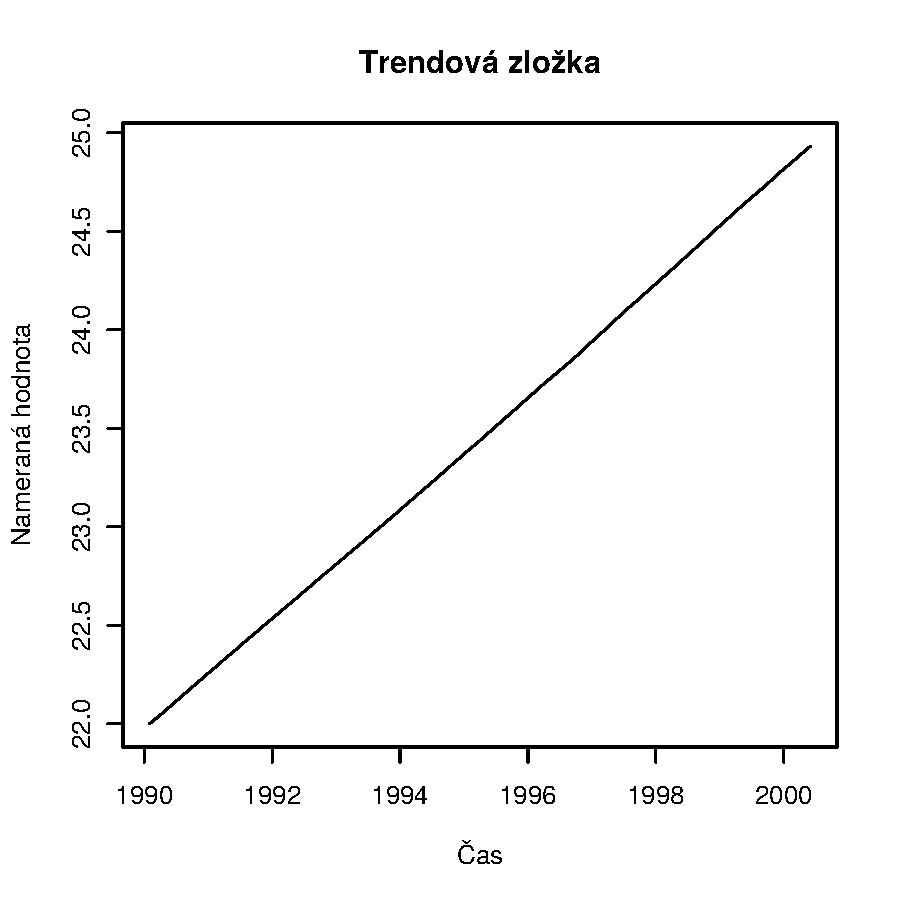
\includegraphics[width=0.65\textwidth]{trend_component.pdf}
  \caption{Príklad trendovej zložky časového radu.}
  \label{fig-trend-comp}
\end{figure}

\paragraph{Cyklická zložka} je spôsobená zmenami, ktoré sa cyklicky opakujú.
Dĺžka periódy je 2 a viac rokov, čo zodpovedá strednodobému časovému horizontu.
Táto zložka je zastúpená najmä pri ekonomických časových radoch napríklad
podnikateľský cyklus pozostávajúci zo 4 fáz, ktoré sa stále
opakujú~\cite{Agrawal2013}.

\begin{figure}[H]
  \centering
  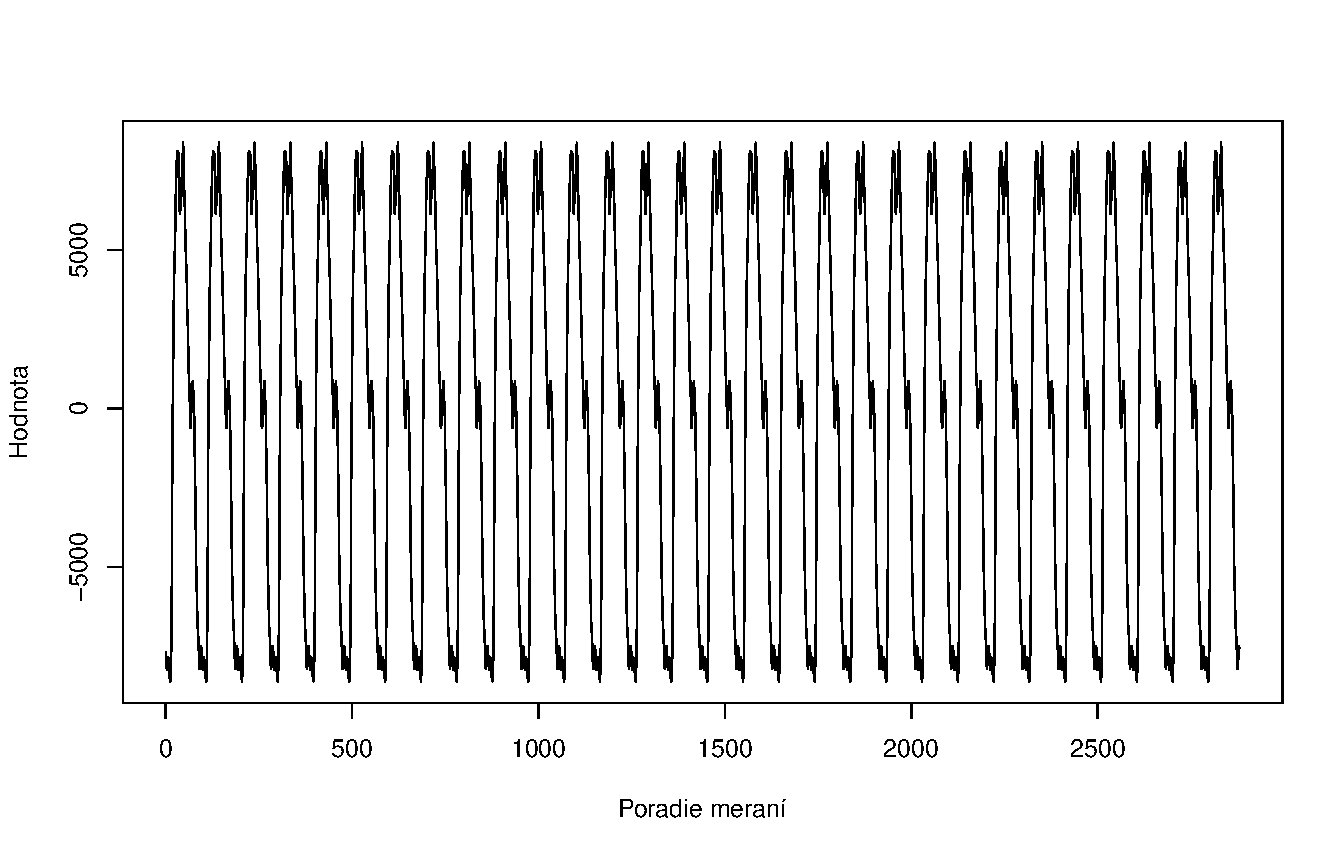
\includegraphics[width=0.7\textwidth]{season_component.pdf}
  \caption{Príklad sezónnej zložky časového radu.}
  \label{fig-season-comp}
\end{figure}

\begin{figure}[H]
  \centering
  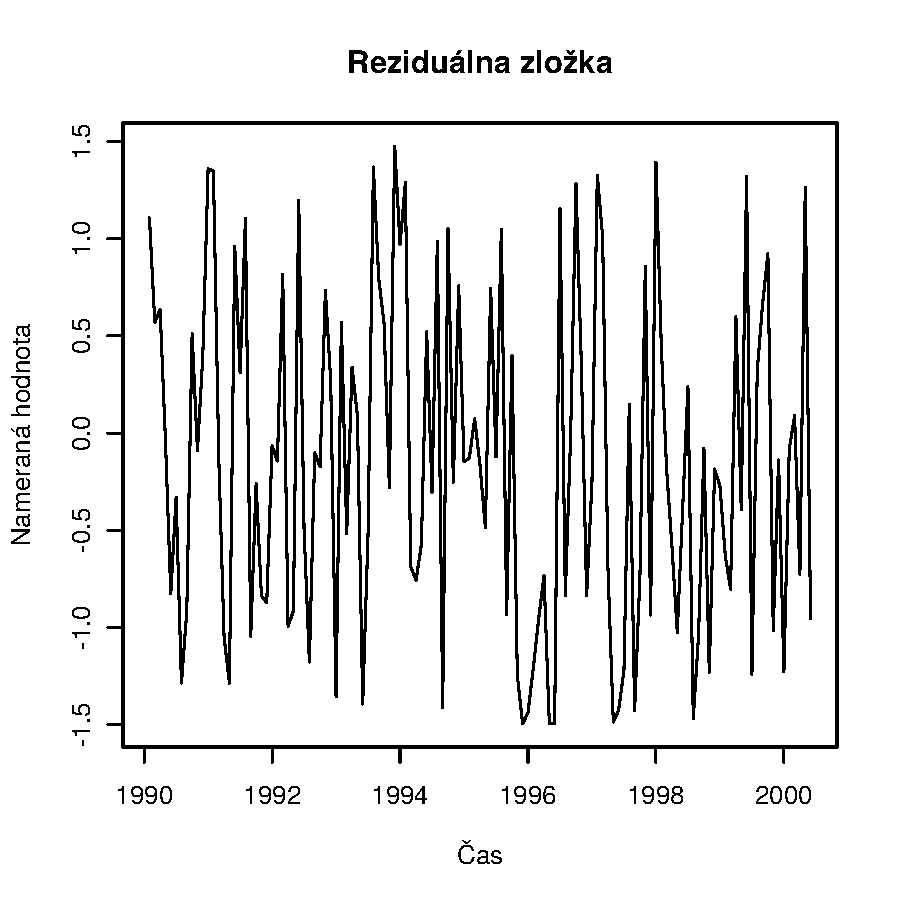
\includegraphics[width=0.7\textwidth]{random_component.pdf}
  \caption{Príklad reziduálnej zložky časového radu.}
  \label{fig-random-comp}
\end{figure}

\paragraph{Sezónna zložka} predstavuje kolísanie časových radov počas ročných
období. Dôležitými faktormi pri tom sú napr. klimatické podmienky, tradície
alebo počasie. Napríklad predaj zmrzliny sa v lete zvyšuje, ale počet
predaných lyžiarskych súprav klesá~\cite{Agrawal2013}.

\paragraph{Reziduálna zložka} predstavuje veličinu, ktorá nemá žiadny
opakovateľný vzor a ani dlhodobý trend. V časových radoch má nepredvídateľný
vplyv na pozorovanú veličinu. V štatistike zatiaľ nie je definovaná metóda jej
merania. Označuje sa aj ako náhodná zložka alebo biely šum. Je spôsobená
nepredvídateľnými a nepravidelnými udalosťami~\cite{Agrawal2013}.

Vo všeobecnosti sa pre tieto 4 zložky používajú 2 rôzne modely. Je to
multiplikatívny model a aditívny model.
\begin{equation}
  \begin{split}
    Y(t) = T(t) \times S(t) \times C(t) \times I(t)
    \\
    Y(t) = T(t) + S(t) + C(t) + I(t)
  \end{split}
  \label{eq-ts-models}
\end{equation}
Vo vzorci~\ref{eq-ts-models} predstavuje $Y(t)$ meranie v čase $t$. Premenné
$T(t)$, $S(t)$, $C(t)$ a $I(t)$ sú zložkami trendu, sezónnosti,
cyklu a náhodnosti. Multiplikatívny model, zobrazený na
obrázku~\ref{fig-multi-model} je založený na predpoklade, že časové rady môžu
byť na sebe závislé a môžu byť ovplyvňované medzi sebou, zatiaľ čo aditívny
model, zobrazený na obrázku~\ref{fig-add-model} predpokladá nezávislosť
zložiek~\cite{Agrawal2013}.

\begin{figure}[!ht]
  \centering
  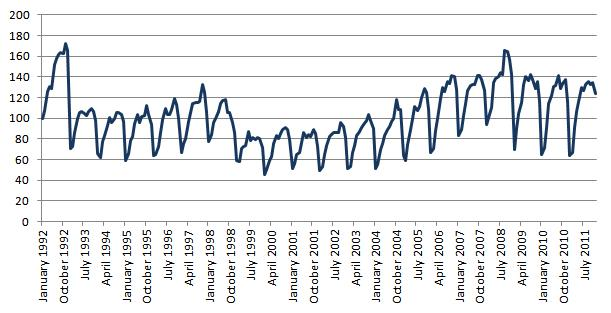
\includegraphics[width=\textwidth]{multi_model.jpg}
  \caption{Príklad multiplikatívneho modelu}
  \label{fig-multi-model}
  \small
  Index stavebnej produkcie Slovenska
\end{figure}

\begin{figure}[!ht]
  \centering
  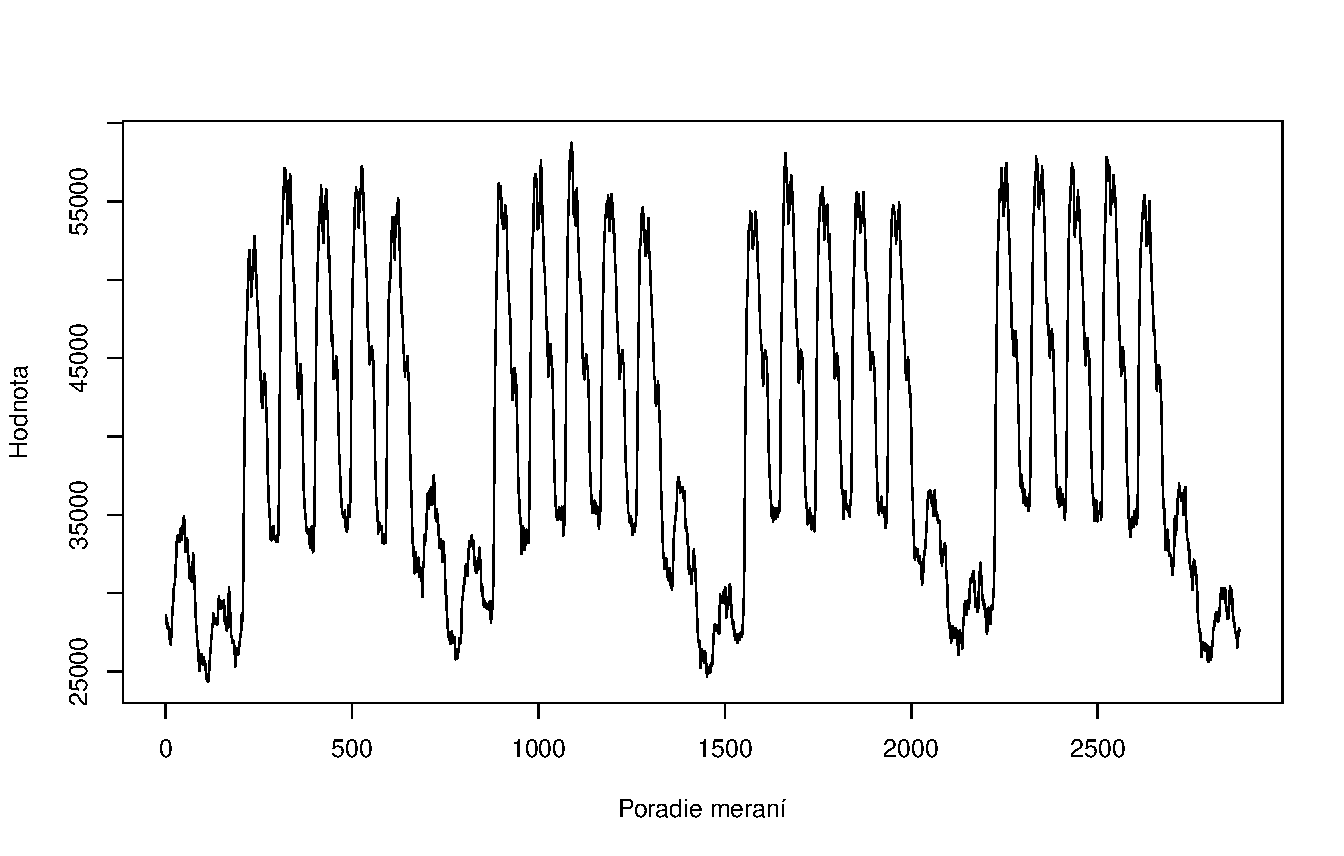
\includegraphics[width=\textwidth]{add_model.pdf}
  \caption{Príklad aditívneho modelu.}
  \label{fig-add-model}
\end{figure}

%-------------------------------------------------------------------------------
%   Analysis of prediction algorithms
%-------------------------------------------------------------------------------

\subsection{Analýza predikčných algoritmov}
Na základe množstva výskumov, ktoré analyzovali predikčné algoritmy, sme si
zvolili reprezentatívnu vzorku algoritmov. Našou snahou bude rôzne predikčné
metódy optimalizovať pomocou optimalizačných algoritmov. Pred tým je potrebné
analyzovať a pochopiť použité predikčné metódy. Taktiež je potrebné
identifikovať ich vstupné parametre, keďže ich neskôr budeme optimalizovať.

%-------------------------------------------------------------------------------
%   Linear regression
%-------------------------------------------------------------------------------

\subsubsection{Lineárna regresia}
Najpoužívanejšia štatistická metóda, ktorá modeluje vzťah závislej premennej
a vysvetľujúcej premennej. Závislú premennú predstavuje veličina, ktorú sa
snažíme predpovedať, čo je v našom prípade spotreba elektrickej energie.
Vysvetľujúca premenná v sebe zahŕňa rôzne faktory, ktoré ovplyvňujú závislú
premennú. Môžeme si pod tým predstaviť deň v týždni, počasie, tradície alebo rôzne
udalosti, ktoré majú vplyv na predpoveď.~\cite{KumarSingh2013, Mahalakshmi2016}.

Predpokladajme typický regresný problém. Dáta pozostávajúce z množiny \textit{n}
meraní majú formát $\left\{(x_1, f(x_1)), ..., (x_n, f(x_n))\right\}$.
Úlohou regresie je odvodiť funkciu $\hat{f}$ z dát, kde
\begin{equation}
  \hat{f} : X \to \mathbb{R} \text{, kde, } \hat{f}(x) = f(x), \forall x \in X,
  \label{eq-regresia}
\end{equation}
Funkcia $f$ vo vzorci~\ref{eq-regresia} reprezentuje reálnu neznámu
funkciu. Algoritmus použitý na odvodenie funkcie $\hat{f}$ sa nazýva
indukčný algoritmus. Funkcia $\hat{f}$ sa nazýva model alebo
prediktor. Obvykle je úlohou regresie minimalizovať odchýlku funkcie pre
štvorcovú chybu, konkrétne strednú štvorcovú chybu MSE~\cite{Mendes-Moreira2012}.

Keďže časový rad pozostáva z viacerých zložiek, môžeme ho zapísať ako funkciu
$L(t)$ definovanú ako
\begin{equation}
  L(t) = Ln(t) + \sum a_i x_i(t) + e(t)
  \label{eq-odber}
\end{equation}
Vo vzorci~\ref{eq-odber} funkcia $Ln(t)$ predstavuje odber elektrickej energie
v čase $t$. Hodnota $a_i$ je odhadovaný pomaly meniaci sa koeficient. Faktory
$x_i(t)$ nezávisle vplývajú na spotrebu elektrickej energie. Môže sa jednať
napr. o počasie alebo zvyky ľudí. Komponent $e(t)$ je biely šum, ktorý má nulovú
strednú hodnotu a pevnú varianciu. Číslo $n$ je počet meraní, obvykle 24
alebo 168, v našom prípade 96 meraní počas jedného dňa~\cite{KumarSingh2013}.

\paragraph{Lineárna regresná analýza} je štatistická metóda používaná na
modelovanie vzťahov, ktoré môžu existovať medzi veličinami. Nachádza súvislosti
medzi závislou premennou a potenciálnymi vysvetľujúcimi premennými. Používame
pri tom vysvetľujúce premenné, ktoré môžu byť namerané súčasne so závislými
premennými alebo aj premenné z úplne iných zdrojov. Regresná analýza môže byť
tiež použitá na zlúčenie trendu a sezónnych zložiek do modelu. Keď je raz model
vytvorený, môže byť použitý na zásah do spomínaných vzťahov alebo, v prípade
dostupnosti vysvetľujúcich premenných, na vytvorenie predikcie~\cite{Liu1992}.

\paragraph{Viacnásobná lineárna regresia} sa snaží modelovať vzťah medzi dvoma
alebo viacerými vysvetľujúcimi premennými a závislou premennou vhodnou
lineárnou rovnicou pre pozorované dáta. Výsledný model je vyjadrený ako funkcia
viacerých vysvetľujúcich premenných~\cite{Grmanova2016}.

Túto funkciu môžeme zapísať ako
\begin{equation}
  Y(t) = V_t a_t + e_t
  \label{eq-multi-regresia}
\end{equation}
Vo vzorci~\ref{eq-multi-regresia} $t$ označuje čas, kedy bolo meranie
uskutočnené. $Y(t)$ predstavuje celkový nameraný odber elektrickej energie.
Vektor $V_t$ reprezentuje hodnoty vysvetľujúcich premenných v čase merania.
Vysvetľujúce premenné môžu predstavovať meteorologické vplyvy, ekonomický
nárast, ceny elektrickej energie či kurzy mien. Chybu modelu v čase $t$
zapíšeme ako $e_t$~\cite{KumarSingh2013, Mahalakshmi2016}.

%-------------------------------------------------------------------------------
%   Stochastic models
%-------------------------------------------------------------------------------

\subsubsection{Stochastické modely}
\label{stochastic}
Tieto metódy časových radov sú založené na predpoklade, že dáta majú vnútornú
štruktúru, ako napr. autokoreláciu, trend či sezónnu varianciu. Najprv sa
precízne zostaví vzor zodpovedajúci dostupným dátam a potom sa na jeho základe
predpovie budúca hodnota veličiny~\cite{KumarSingh2013}.

\paragraph{Autoregresný model} predpovedá budúcu hodnotu premennej ako súčet
lineárnej kombinácie $p$ predchádzajúcich meraní, náhodnej chyby a konštanty.
V literatúre sa označuje ako AR (autoregressive model). Matematicky môžeme
autoregresný model zapísať ako
\begin{equation}
  y_t = c + \sum_{i=1}^{p} \varphi_i y_{t-i} + \varepsilon_t
  \label{eq-ar}
\end{equation}
Vo vzorci~\ref{eq-ar} hodnota $y_t$ predstavuje predpovedanú hodnotu
v čase $t$. Náhodnú chybu v čase $t$ zapíšeme ako $\varepsilon_t$. Hodnoty
$\varphi_i$ sú parametre modelu a $c$ je konštanta. Konštantou $p$ označujeme
rad modelu~\cite{Agrawal2013}.

\paragraph{Model kĺzavého priemeru} na rozdiel od autoregresného modelu používa
ako vysvetľujúce premenné chyby predchádzajúcich meraní a nie priamo hodnoty.
V literatúre sa označuje ako MA (moving average). Matematicky môžeme tento
vzťah zapísať ako
\begin{equation}
  y_t = \mu + \sum_{j=1}^{q} \Theta_j \varepsilon_{t-j} + \varepsilon_t
  \label{eq-ma}
\end{equation}
Vo vzorci~\ref{eq-ma} hodnota $y_t$ predstavuje strednú hodnotu
postupnosti meraní v čase $t$. Hodnoty $\Theta_j$ sú parametre modelu
a konštantou $q$ označujeme rad modelu. Vychádzame z predpokladu, že náhodná
zložka $\varepsilon_t$ je biely šum, čo je rovnomerne distribuovaná náhodná
premenná, ktorá má nulovú strednú hodnotu a konštantnú varianciu
$\sigma^2$~\cite{Agrawal2013}.

\paragraph{Autoregresívny model kĺzavého priemeru} reprezentuje súčasnú hodnotu
časového rádu lineárne na základe jeho hodnôt a hodnôt bieleho šumu
v predchádzajúcich periódach. V literatúre sa označuje ako ARMA (autoregressive
moving average)~\cite{KumarSingh2013}.

Ide o kombináciu autoregresie (AR) a kĺzavého priemeru (MA), vhodnú pre
modelovanie jednorozmerných časových radov. Matematicky môžeme reprezentovať
tento model ako súčet predchádzajúcich modelov
\begin{equation}
  y_t = c + \varepsilon_t + \sum_{i=1}^{p} \varphi_i y_{t-i}  \sum_{j=1}^{q} \Theta_j \varepsilon_{t-j}
  \label{eq-arma}
\end{equation}
Rad modelu určuje $p$ a $q$~\cite{Agrawal2013}.

\paragraph{Autoregresívny integrovaný model kĺzavého priemeru} je
generalizáciou modelu ARMA. V literatúre sa označuje ako ARIMA (autoregressive
integrated moving average). Modely typu ARMA môžu byť použité iba na statické
časové rady. Mnoho časových radov v praxi vykazuje nestatické správanie a napr.
tie, ktoré obsahujú komponenty trendu a sezónnosti. Kvôli tomu bol navrhnutý
model ARIMA, ktorý zahŕňa v sebe aj prípady nestatických časových radov.
Z nestatických časových radov sa vytvárajú statické pomocou konečného počtu
derivovaní dátových bodov. Vzniká tak matematický model, ktorý môžeme zapísať
ako
\begin{equation}
  \Big( 1 - \sum_{i=1}^{p} \varphi_i L^i \Big) (1-L)^d y_t = \Big( 1 + \sum_{j=1}^{q} \Theta_j L^j \Big) + \varepsilon_t
  \label{eq-arima}
\end{equation}
Vzorec~\ref{eq-arima} môžeme zapísať aj jednoduchšie a to
\begin{equation}
  \varphi(L) (1-L)^d y_t = \Theta(L) \varepsilon_t
  \label{eq-arima-short}
\end{equation}
Vo vzorci~\ref{eq-arima} predstavujú premenné $p$, $d$ a $q$ rad autoregresného
modelu, modelu kĺzavého priemeru a integrovaného modelu. Hodnota $d$ zodpovedá
stupňu derivovania, zvyčajne je rovná 1. V prípade, že $d=0$ dostaneme klasický
ARMA model. Rovnakým spôsobom vieme dostať modely AR a MA~\cite{Agrawal2013}.

%-------------------------------------------------------------------------------
%   Support vector regression
%-------------------------------------------------------------------------------

\subsubsection{Regresia založená na podporných vektoroch}
Regresia založená na podporných vektoroch a metóda podporných vektorov je
založená na štatistickej teórií učenia, nazývanej aj VC teória, podľa svojich
autorov, Vapnik a Chervonenkisa. Táto predikčná metóda poskytuje malý počet
voľných parametrov. Garantuje konvergenciu k ideálnemu riešeniu a môže byť
výpočtovo efektívna~\cite{Sapankevych2009}.

Metóda podporných vektorov je použitá na množstvo úloh strojového učenia ako je
rozoznávanie vzorov, klasifikácia objektov a v prípade predikcií časových
radov to je regresná analýza. Regresia založená na podporných vektoroch je
postup, ktorého funkcia je predpovedaná pomocou nameraných dát, ktorými je
metóda podporných vektorov natrénovaná. Toto je odklon od tradičných predpovedí
časových radov v zmysle, že metóda podporných vektorov nepoužíva žiadny model,
ale predikciu riadia samotné dáta~\cite{Sapankevych2009}.

Uvažujme množinu trénovacích dát
${(x_1, y_1), (x_2, y_2), ..., (x_n, y_n)} \subset \chi \times \mathbb{R}$, kde
v našom prípade hodnota $x_i$ predstavuje odber elektrickej energie v čase $i$
a množina $\chi$ označuje vstupnú množinu dát. Úlohou algoritmu je nájsť
funkciu  $f(x_i)$, pre ktorú hodnota $\varepsilon$ nadobúda pre všetky
trénovacie dáta čo najväčšie hodnoty oproti $y_i$ a súčasne nadobúda
najmenšie možné hodnoty menšie ako $\varepsilon$~\cite{Smola2004}.

Matematicky môžeme túto lineárnu zapísať ako
\begin{equation}
  f(x) = \langle w, x \rangle +  b
  \label{eq-svr}
\end{equation}
Vo vzorci~\ref{eq-svr} platí $w \in \chi$ a $b \in \mathbb{R}$. Výsledok
vektorového súčinu $\langle w, x \rangle$ sa nachádza v množine $\chi$. Našou
snahou je dosiahnuť čo najmenšiu hodnotu $w$. Zabezpčiť to môžeme
minimalizovaním hodnoty $|| w ||^2 = \langle w, w \rangle$. Pri cieli
minimalizovať hodnotu $\frac{1}{2} || w ||^2$, môžeme opisovaný problém zapísať
ako
\begin{equation}
  \begin{cases}
    y_i - \langle w, x_i \rangle - b \leq \varepsilon \\
    \langle w, x_i \rangle + b - y_i \leq \varepsilon \\
  \end{cases}
  \label{eq-svr-min}
\end{equation}
Predpokladom pre vzorec~\ref{eq-svr-min} je, že funkcia $f$ existuje pre všetky
páry $(x_i, y_i)$ s presnosťou~$\varepsilon$~\cite{Smola2004}.

%-------------------------------------------------------------------------------
%   Decision trees
%-------------------------------------------------------------------------------

\subsubsection{Rozhodovacie stromy}
Rozhodovacie stromy sú jednou z najrozšírenejších učiacich metód. Používajú sa
najmä na klasifikáciu, ale v súčasnosti sa využívajú aj na regresiu.
Rozhodovací strom je reprezentovaný ako množina uzlov a im prislúchajúcich
hrán. Uzly reprezentujú atribúty a výstupné hrany sú vždy označené konkrétnou
hodnotou pre atribút, z ktorého vychádzajú. Rozhodovanie začína v koreni stromu
a končí po dosiahnutí listového uzla. Pre riešenie jedného problému je možné
vytvoriť stromy s rôznym počtom a usporiadaním uzlov. Najlepším riešením je
strom s najmenším počtom rozhodovacích uzlov~\cite{Merz1998}.

Hlavnou výhodou rozhodovacích stromov oproti ostatným modelom je, že strom
produkuje model, ktorý je reprezentovateľný ako pravidlá alebo logické výroky.
Taktiež klasifikácia sa môže vykonávať bez komplikovaných výpočtov. Táto
technika môže byť použitá ako na kategorické premenné tak aj na spojité.
Rozhodovacie stromy neposkytujú také dobré výsledky pre nelineárne dáta ako
neurónové siete. Vo všeobecnosti je táto metóda vhodnejšia pre predpovedanie
kategorických dát alebo na dáta, ktoré v sebe obsahujú viditeľný
trend~\cite{Tso2007}.

%-------------------------------------------------------------------------------
%   Regression trees
%-------------------------------------------------------------------------------

\paragraph{Regresný rozhodovací strom} obsahuje odozvový vektor $Y$
reprezentujúci odozvu hodnôt ku každému meraniu v matici $X$. Vetvy sú
rozdeľované na základe štvorcového zostatkového minimalizačného algoritmu.
Ten zabezpečuje, že očakávaný súčet variancií dvoch uzlov bude minimalizovaný.
Algoritmus tak nájde optimálnu podmienku rozdelenia uzlu na jeho
potomkov~\cite{Bel2009}.

Priradením hodnoty 1 pre triedu $k$ a hodnoty 0 pre ostatné triedy, získame
varianciu rovnú $p(k|t)[1 - p(k|t)]$. Sčítaním $K$ tried získame funkciu
\begin{equation}
  i(t) = 1 - \sum_{k = 1}^K p^2 (k|t)
  \label{eq-tree-impurity}
\end{equation}
Tým sme vytvorili maximálny strom, čo znamená, že uzly sa rozdeľovali až do
posledného merania, ktoré sa nachádzalo v trénovacej množine. Maximálny strom
sa tak môže stať veľmi veľkým~\cite{Bel2009}.

Jedným z najpoužívanejších algoritmov na rozdeľovanie uzlov sa nazýva index
Gini alebo rozhodovacie pravidlo Gini. Tento algoritmus zapíšeme ako
\begin{equation}
  i(t) = \sum_{k \neq l} p(k|t) p(l|t)
  \label{eq-tree-gini}
\end{equation}
Vo vzorci~\ref{eq-tree-gini} predstavujú $k$ a $l$ indexy tried o 1 po $K$ a
$p(k|t)$ označuje podmienenú pravdepodobnosť triedy $k$ za predpokladu, že
aktuálny uzol je uzol $t$. Aplikovaním Gini algoritmu nájdeme v trénovacej
množine najväčšiu triedu, ktorú odizolujeme od ostatných dát~\cite{Bel2009}.

%-------------------------------------------------------------------------------
%   Random forest
%-------------------------------------------------------------------------------

\paragraph{Náhodné lesy} sú kombináciou predpovedí stromov. Každý strom závisí
od hodnoty náhodného vektora s rovnakým rozdelením. Chyba lesu závisí od sily
jednotlivých stromov a koreláciou medzi nimi. Náhodný les môžeme definovať ako
klasifikátor pozostávajúci z množiny stromov $\{h(x, \Theta_k), k=1, 2, ... \}$,
kde $\{\Theta_k\}$ sú nezávislé rovnomerne distribuované náhodné vektory a každý
strom sa podieľa hlasom na voľbe triedy vstupu $x$. S nárastom počtu stromov
hodnota $\{\Theta_k\}$ konverguje k určitému bodu. Tým je zabezpečené, že
náhodné lesy sa s pridávajúcim počtom stromov nepretrénujú, ale veľkosť chyby
sa postupne ustáli. Pri výbere náhodného vektora sa snažíme pri zachovaní jeho
sily minimalizovať koreláciu, čím zvyšujeme presnosť celého
výpočtu~\cite{Breiman2001}.

Väčšinou sú náhodné lesy používané na klasifikačné problémy, avšak je možné ich
aplikovať aj na regresiu. Regresné náhodné lesy sú tvorené rastom stromov
závislých na náhodnom vektore $\{\Theta\}$. Prediktor stromu $h(x, \Theta)$
nadobúda číselné hodnoty na rozdiel od štítkov tried ako je to pri klasifikačných
problémoch. Predpokladáme trénovaciu množinu, ktorá je nezávislou distribúciou
náhodného vektora $Y, X$. Potom môžeme strednú štvorcovú generalizačnú chybu
pre číselný prediktor $h$ matematicky zapísať ako
\begin{equation}
  E_{X, Y} (Y - h(X))^2
  \label{eq-random-error}
\end{equation}
Prediktor náhodného lesu je tvorený priemerom $k$ stromov, čo zapíšeme ako
$h(x, \Theta_k)$~\cite{Breiman2001}.

%-------------------------------------------------------------------------------
%   Neural networks
%-------------------------------------------------------------------------------

\subsubsection{Neurónové siete}
Návrh neurónových sietí je inšpirovaný neurofyziológiou ľudského mozgu. Model
je analytická technika modelujúca procesy učenia v kognitívnych systémoch
a neurologických funkciách mozgu. Má schopnosť predpovedať budúcu hodnotu
merania konkrétnej premennej na základe hodnôt z predchádzajúcich meraní. Tento
proces sa inak nazýva aj učenie z existujúcich dát. Tok v neurónovej sieti
preteká cez jednotlivé neuróny. Na obrázku~\ref{fig-neuron} môžeme vidieť
príklad takéhoto neurónu~\cite{Tso2007}.

\begin{figure}[!ht]
  \centering
  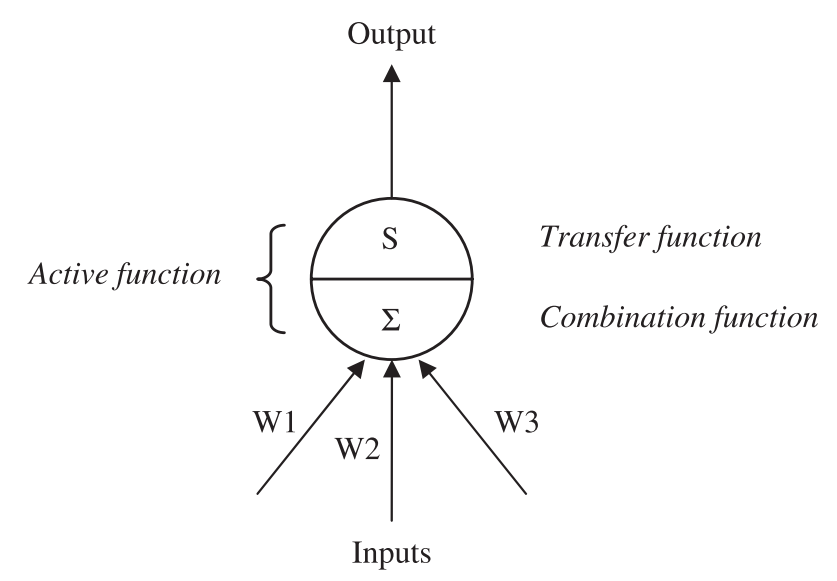
\includegraphics[width=0.6\textwidth]{neuron.png}
  \caption{Príklad neurónu v neurónovej sieti.}
	\source{Tso, G. K.; Yau, K. K.: Predicting electricity energy consumption:
					A comparison of regression analysis, decision tree and neural
					networks. Energy, ročník 32, č. 9, 2007: s. 1761 – 1768, ISSN 0360-5442,
					doi:http://dx.doi.org/10.1016/j.energy.2006.11.010.
					URL http://www.sciencedirect.com/science/article/pii/S0360544206003288}
  \label{fig-neuron}
\end{figure}

Neurónová sieť predstavuje orientovaný graf uzlov. Uzol neurónovej
siete sa nazýva neurón. Každý uzol počíta svoj výstup na základe vstupov od
susedných uzlov. Výpočet prebieha aplikovaním funkcie, ktorá sa nazýva sigmoid,
na vážený súčet vstupov~\cite{Gruau1994}.

Trénovanie siete je proces nastavovania, čo najlepších váh na vstupy
jednotlivých neurónov. Chyba neurónovej siete sa najčastejšie počíta pomocou
spätnej propagácie (backpropagation), čím dostaneme rast chyby pre danú
neurónovú sieť~\cite{Tso2007}.

Je veľa typov neurónových sietí napríklad viacvrstvové perceptónové siete,
samoriadiace siete, siete s viacerými skrytými vrstvami, alebo aj viacvrstvové
spätne propagované neurónové siete, pričom príklad takejto siete môžeme vidieť
aj na obrázku~\ref{fig-neural-network}. V každej skrytej vrstve je množstvo
neurónov. Hlavnou výhodou je, že väčšina sietí nepotrebuje model. Na druhej strane,
trénovanie obvykle zaberá veľa času. Výstupom siete je lineárna rovnica váh
prepojených so vstupom~\cite{KumarSingh2013}.

\begin{figure}[!ht]
  \centering
  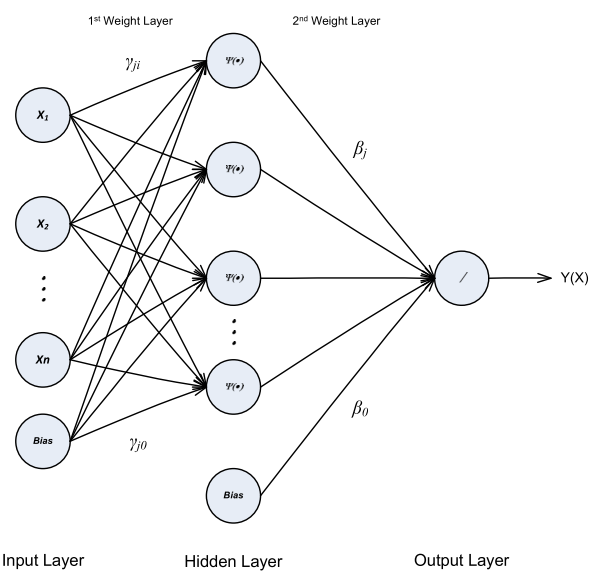
\includegraphics[width=\textwidth]{neural_network.png}
  \caption{Príklad viacvrstvovej spätne propagovanej neurónovej siete.}
	\source{Kennedy, J.; Eberhart, R.: Particle swarm optimization. In Neural
					Networks, 1995. Pro-ceedings., IEEE International Conference on,
					ročník 4, Nov 1995, s. 1942–1948 vol.4, doi:10.1109/ICNN.1995.488968.}
  \label{fig-neural-network}
\end{figure}

\textbf{Viacvrstvový perceptón} je jednou z najpoužívanejších neurónových
sietí. Pozostáva z uzlov a im prislúchajúcim hranám. Uzly sú zoskupované do
rôznych vrstiev. Prvá vrstva je vstupná vrstva, kde počet $d$ označuje počet
vstupných parametrov vstupujúcich do siete. Táto vrstva je následne prepojená
hranami so skrytou vrstvou pozostávajúcou z $h$ uzlov. Tá je potom prepojená
s výstupnou vrstvou s $c$ uzlami. Kvôli tomu sa tieto siete zvyknú označovať aj
ako dopredné siete~\cite{Merz1998}.

Elementy skrytých a výstupných vrstiev sú umelé neuróny pozostávajúce z uzlov,
viacerých vstupujúcich a jednou výstupnou hranou. Funkciou neurónu je
transformovať lineárnu kombináciu vstupov pomocou nelineárnej aktivačnej
funkcie, čiže každú vstupnú hranu prenásobiť jej váhou a výsledok týchto súčinov
sčítať. Tak dostaneme pre neurón $j$ vzorec~\ref{eq-linear-combination}
opisujúci lineárnu kombináciu vstupov $a_j$
\begin{equation}
  a_j = \sum_{i=1}^{d} w_{ji} x_i
  \label{eq-linear-combination}
\end{equation}
Pričom váha $w_{ji}$ označuje váhu medzi neurónom $i$ na vstupnej vrstve
a neurónom $j$ na skrytej vrstve~\cite{Merz1998}.

Aktivovanie neurónu $j$ závisí od jeho aktivačnej funkcie $g(a_j)$. Jednu
z najpoužívanejších aktivačných funkcií, logistickú sigmoidnú funkciu, môžeme
matematicky zapísať ako
\begin{equation}
  g(a) \equiv \frac{1}{1 + exp(-a)}
  \label{eq-sigmoid-function}
\end{equation}
Je zrejmé, že funkcia zo vzorca~\ref{eq-sigmoid-function} vracia hodnoty
v rozmedzí $(0,1)$~\cite{Merz1998}.

%-------------------------------------------------------------------------------
%   Analysis of optimizing algorithms
%-------------------------------------------------------------------------------

\subsection{Analýza optimalizačných algoritmov}
Optimalizačné algoritmy, ktoré majú potenciál nájsť globálne alebo lokálne
riešenie problému. Lokálne optimalizácie, nazývané aj vyhľadávacie algoritmy,
sa pokúšajú nájsť lokálne minimum v okolí štartovacieho riešenia. Väčšina
týchto algoritmov je deterministická. Pri hľadaní minima používajú
vyhodnocovaciu funkciu, na základe ktorej aktualizujú doterajšie riešene.
Z nových možných riešení je najlepšie to s najnižšou hodnotou, čiže to, ktoré
je najlacnejšie. Kvôli tejto vlastnosti sa zvyknú tieto algoritmy označovať aj
ako nenásytné algoritmy (greedy algorithms). Spravidla tieto algoritmy nenájdu
globálne minimum v prípade, že sa nachádza ďalej od štartovacieho riešenia ako
nejaké lokálne minimum~\cite{Sen1995}.

Na druhej strane, optimalizačné algoritmy s potenciálom nájdenia globálneho
minima nachádzajú riešenie, ktoré postupne konverguje k optimálnemu riešeniu.
To ale nie je algoritmami úplne garantované. Algoritmy s globálnym
potenciálom majú väčší prehľad o svojom okolí, a preto uviaznutie v lokálnom
minime je zriedkavé~\cite{Sen1995}.

Nasledujúca tabuľka~\ref{tab-bio} zobrazuje rozdelenie algoritmov
s potenciálom nájdenia globálneho minima. Algoritmy sú prírodne inšpirované
a ich ďalšie delenie vyplýva zo spoločných znakov, na ktorých sú založené.

\begin{table}[ht]
  \centering
  \caption{Rozdelenie rozdelenie vybraných prírodne inšpirovaných algoritmov.}
	\source{Goel, L.; Gupta, D.; Panchal, V. K.; aj.: Taxonomy of nature inspired
					computational intelligence: A remote sensing perspective. In 2012
					Fourth World Congress on Nature and Biologically Inspired Computing
					(NaBIC), Nov 2012, s. 200–206, doi:10.1109/NaBIC.2012.6402262.}
  \label{tab-bio}
  % \begin{tabular}{|p{34mm}|p{34mm}|p{34mm}|p{34mm}|}
  \begin{tabular}{|l|l|l|l|}
    \hline
    \multicolumn{1}{|c|}{\textbf{\begin{tabular}[c]{@{}c@{}}Model ľudskej \\ mysle\end{tabular}}} & \multicolumn{1}{c|}{\textbf{\begin{tabular}[c]{@{}c@{}}Umelé imunitné \\ systémy\end{tabular}}} & \multicolumn{1}{c|}{\textbf{\begin{tabular}[c]{@{}c@{}}Rojová \\ inteligencia\end{tabular}}} & \multicolumn{1}{c|}{\textbf{\begin{tabular}[c]{@{}c@{}}Ostatné napr. \\ prírodné úkazy\end{tabular}}} \\ \hline
    Teória fuzzy množín                                                                           & Genetický algoritmus                                                                            & \begin{tabular}[c]{@{}l@{}}Optimalizácia \\ kolóniu mravcov\end{tabular}                     & Tektonické dosky                                                                                      \\
    Teória približných množín                                                                     & Umelé neurónové siete                                                                           & \begin{tabular}[c]{@{}l@{}}Optimalizácia \\ rojom častíc\end{tabular}                        & Veľký kolaps                                                                                          \\
    Granulárne výpočty                                                                            & Celulárný automat                                                                               & \begin{tabular}[c]{@{}l@{}}Inteligentná \\ kvapka vody\end{tabular}                          & Oceánske prúdy                                                                                        \\
    Predbežné výpočty                                                                             & Membránové výpočty                                                                              & \begin{tabular}[c]{@{}l@{}}Včelí zhlukovací \\ algoritmus\end{tabular}                       & Prílivové vlny                                                                                        \\
                                                                                                  &                                                                                                 & \begin{tabular}[c]{@{}l@{}}Vyhľadávanie \\ kukučkou\end{tabular}                             & Sopečné erupcie                                                                                       \\
                                                                                                  &                                                                                                 &                                                                                              & Zemetrasenie                                                                                          \\
    \hline
  \end{tabular}
\end{table}

%-------------------------------------------------------------------------------
%   Genetic algorithms
%-------------------------------------------------------------------------------

\subsubsection{Genetický algoritmus}
Genetický algoritmus patrí medzi prírodne inšpirované algoritmy patriace do
triedy umelých imunitných systémov. Genetický algoritmus je stochastický
optimalizačný algoritmus, ktorého úlohou je nájdenie globálneho riešenia pre
zadaný problém, čiže sa nestane, že riešenie spadne do lokálne minima a nenájde
sa tak optimálne riešenie. Od tradičných algoritmov sa líšia hlavne v počte
riešení, ktoré sú kandidátmi na najlepšie riešenie. Tradičné vyhľadávacie
algoritmy prehľadávajú dôkladne iba jedno riešenie, zatiaľ čo genetické
algoritmy hlbšie spracujú viacero kandidátov naraz. Každý kandidát na optimálne
riešenie problému je reprezentovaný dátovou štruktúrou, ktorú označujeme pojmom
jedinec. Súbor jedincov tvorí populáciu. Začiatok procesu začína náhodnými
riešeniami populácie, ktorý sa postupne vylepšuje~\cite{Chavan2015}.

Vytvorenie novej generácie sa vykonáva pomocou genetických operátorov:
a to selekciou, krížením a mutáciou. Proces selekcie vyberie kvalitnejšie
chromozómy, ktoré prežijú a vyskytnú sa tak aj v ďalšej
generácii~\cite{Simonova2007}.

Pri genetických algoritmoch sa zavádzajú pojmy ako chromozóm, fitness funkcia,
kríženie, elitárstvo, operátor reprodukcie či mutácie~\cite{Chavan2015}.

\paragraph{Chromozóm} je pomenovanie pre jedinca. V literatúre sa tiež zvykne
používať označenie kandidát~\cite{Arun2016}.

\paragraph{Inicializácia} je proces, ktorý po vygenerovaní generácie priradí
kandidátom náhodné hodnoty. Pri prehľadávaní dvojrozmerného priestoru to budú
náhodné hodnoty oboch súradníc~\cite{Lazinica2009}.

\paragraph{Fitness funkcia} je funkcia určujúca efektívnosť chromozómu. Každý
jedinec v množine je ohodnotený pomocou tejto funkcie, ktorá vracia číselnú
reprezentáciu riešenia, čiže ako dobre daný kandidát vyriešil zadaný problém.
Pri hľadaní optimálneho riešenia sa porovnáva hodnota fitness funkcie aktuálneho
riešenie s hodnotou funkcie cieľového riešenia, ale vo všeobecnosti, čím je
hodnota väčšia, tým je kandidátovo riešenie
lepšie~\cite{Chavan2015, Lazinica2009, Simonova2007}.

\paragraph{Operátor reprodukcie} je obvykle prvý operátor, ktorý sa uplatní na
populáciu. Operátor náhodne vyberie reťazce z dvoch chromozómov na
párenie~\cite{Chavan2015}.

\paragraph{Kríženie} je operátor kombinácie. Kríženie vykonáva výmenu blokov
chromozómov. Z druhého chromozómu je vybraný reťazec náhodnej veľkosti, ktorý
sa vymení s rovnako dlhým reťazcom z prvého chromozómu.
V tabuľke~\ref{tab-crossing} je tento proces znázornený
graficky~\cite{Chavan2015}.

\begin{table}[H]
  \centering
  \caption{Proces vytvorenia novej generácie z rodičovských chromozómov.}
  \label{tab-crossing}
  \begin{tabular}{p{4cm}l|l|l}
    rodič č. 1      &  0110 & 0101  0010 & 0011  \\
    rodič č. 2      &  1100 & 1101  1110 & 1111  \\
    \hline
    potomok č. 1    &  0110 & 1101  1110 & 0011  \\
    potomok č. 2    &  1100 & 0101  0010 & 1111  \\
  \end{tabular}
\end{table}

Vzniká problém ako čo najvhodnejšie určiť bod kríženia a vybrať tak
najkvalitnejšie bloky chromozómu. Kvôli tomu je potrebné definovať nový element
nazývaný väzba, označovaný ako $d_i$
\begin{equation}
  d_i = \frac{a_i + a_{i+1}}{2}
  \label{eq-crossing}
\end{equation}
Za predpokladu, že chromozóm reprezentujeme ako maticu veľkosti $1 \times N$,
potom väzbu definovanú vzorcom \ref{eq-crossing} môžeme reprezentovať ako
maticu $1 \times (N-1)$. Vypočítaním priemeru susedných hodnôt aj pre cieľovú
maticu a nájdením priemeru matice, určíme body kríženia. Chromozóm rozdelíme na
miestach, kde je väzba, čo najmenšia~\cite{Simonova2007}.

\paragraph{Elitárstvo} je proces pridávania chromozómov s najlepšou hodnotou
funkcie fitness priamo do ďalšej populácie. Zaisťuje to, že najlepšie riešenie
budúcej generácie bude vždy lepšie alebo pri najhoršom rovnaké, ako najlepšie
riešenie predchádzajúcej generácie~\cite{Deolekar2016}.

\paragraph{Operátor mutácie} sa vykoná po vykonaní operátora reprodukcie.
Mutácia chromozómu väčšinou predstavuje operáciu, ktorá s nízkou
pravdepodobnosťou invertuje jeden bit v chromozóme~\cite{Chavan2015}.

\paragraph{Princíp genetického algoritmu} môžeme znázorniť v nasledujúcom
pseudokóde~\cite{Chavan2015}
\begin{algorithm}
  \caption{Pseudokód genetického algoritmu}
  \begin{algorithmic}[1]
    \State Náhodne inicializovanie jedincov
    \State Vyhodnotenie fitness funkcie pre každého jedinca \label{ga-fitness}
    \State Výber jedincov pre ďalšiu populáciu na základe fitness funkcie
    \State Kríženie jedincov
    \State Mutovanie jedincov
    \State Ak bolo nájdené žiadané optimálne riešenie pokračuj, inak návrat na krok \ref{ga-fitness}
    \State Vráť optimálne riešenie
  \end{algorithmic}
\end{algorithm}

Veľkou výhodou genetického algoritmu je, že mutácia predchádza skĺznutiu do
lokálnych miním a kombinácia chromozómov vedie k rýchlemu približovaniu
sa k optimálnemu riešeniu. Napriek týmto výhodám, majú genetické algoritmy aj
niekoľko nevýhod~\cite{Deolekar2016}.
\begin{itemize}
  \item Reprezentovanie kandidátov je príliš obmedzujúce
  \item Mutácia a kríženie sú v súčasnosti aplikovateľné iba na chromozómy
        reprezentované bitovým reťazcom alebo číslami
  \item Definovanie fitness funkcie je často netriviálnou záležitosťou
        a jej generalizácia je náročná
\end{itemize}

%-------------------------------------------------------------------------------
%   Grey wolf optimizer
%-------------------------------------------------------------------------------

\subsubsection{Optimalizácia svorkou divých vlkov}
Algoritmus je založený na správaní vlka sivého, ktorý je na vrchole
potravinového reťazca a preferuje život vo svorke. Lov pozostáva zo stopovania,
prenasledovania, približovania sa, obkľúčenia koristi a útokom na korisť. Vlkov
vo svorke možno rozdeliť do niekoľkých skupín.
V obrázku~\ref{fig-wolf-hierarchy} je znázornená hierarchia týchto
skupín~\cite{Seeley1991}.

\begin{figure}[!ht]
  \centering
  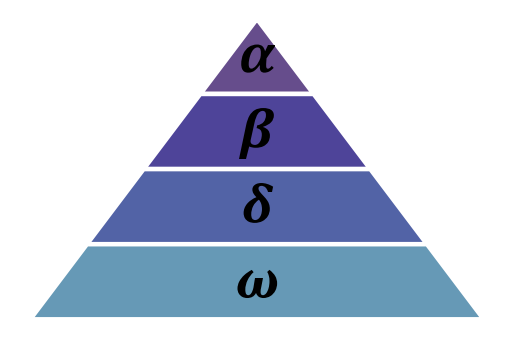
\includegraphics[width=0.5\textwidth]{wolf_hierarchy.png}
  \caption{Hierarchia vlkov vo svorke.}
	\source{Seeley, T. D.; Camazine, S.; Sneyd, J.: Collective decision-making in
					honey bees: how colonies choose among nectar sources. Behavioral
					Ecology and Sociobiology, ročník 28, č. 4, 1991: s. 277–290, ISSN
					1432-0762, doi:10.1007/BF00175101. URL http://dx.doi.org/10.1007/BF00175101}
  \label{fig-wolf-hierarchy}
\end{figure}

\paragraph{Alfa vlky} sú vodcami svorky. Ich úlohou je robiť rozhodnutia
ohľadom lovu, miesta na spanie či času zobudenia. Tieto príkazy diktujú svorke,
avšak bolo pozorované aj demokratické správanie, kedy alfa vlky nasledovali
ostatných členov svorky. Všetky vlky uznávajú postavenie alfy vo svorke.
Zaujímavosťou je, že vodcom nemusí byť najsilnejší jedinec, ale môže to
byť aj jedinec najlepší v organizovaní svorky~\cite{Seeley1991}.

\paragraph{Beta vlky} sú druhým stupňom v hierarchii, podriadené alfa vlkom,
ktorým pomáhajú v rozhodovaní a organizácií. Sú najlepšími kandidátmi na alfu
v prípade úmrtia alebo zostarnutia alfa jedincov. Hrajú rolu radcu a ďalej
distribuujú príkazy a vracajú sa s odozvou na ne~\cite{Seeley1991}.

\paragraph{Delta vlky} inak nazývané aj podriadené, zastupujú vo svorke
úlohy prieskumníkov, strážcov, starejších, lovcov či opatrovateľov.
Prieskumníci hliadkujú hranice a varujú svorku pred nebezpečím. Strážcovia
sa starajú o bezpečie svorky. Starejší sú skúsenými vlkmi, ktorí boli na pozícii
alfa alebo beta. Lovci pomáhajú alfa a beta vlkom pri love. Opatrovatelia sa
starajú o slabé, choré alebo zranené jedince~\cite{Seeley1991}.

\paragraph{Omega vlky} majú najnižšiu hodnosť vo svorke. Hrajú rolu obetných
baránkov, ktoré sa podrobia ostatným. K potrave sa dostanú ako úplne posledné.
Aj keď sa možno javí ich postavenie zbytočné, boli pozorované prípady, kedy ich
strata spôsobila vo svorke nedorozumenia~\cite{Seeley1991}.

\paragraph{Spoločenská hierarchia} reprezentovaná matematickým modelom,
označuje najvhodnejšie riešenie ako alfa, druhé a tretie najvhodnejšie ako beta
resp. delta. Riešenia ostatných kandidátov označujeme ako omega. Algoritmus
optimalizácie (v prírode lovu) je vedený alfa, beta a delta kandidátmi, ktorí
sú nasledovaní kandidátmi omega~\cite{Seeley1991}.

\paragraph{Obkľúčenie koristi} jednotlivými vlkmi $\alpha$, $\beta$ a $\delta$
môžeme matematicky vyjadriť nasledujúcimi rovnicami
\begin{equation}
  \vec{D_\alpha} = | \vec{C_1} \cdot \vec{X_\alpha} - \vec{X} |
  \label{eq-prey-alpha}
\end{equation}

\begin{equation}
  \vec{X_1} = \vec{X_\alpha} - \vec{A_1} \cdot \vec{D_\alpha}
  \label{eq-prey-x1}
\end{equation}

\begin{equation}
  \vec{D_\beta} = | \vec{C_2} \cdot \vec{X_\beta} - \vec{X} |
  \label{eq-prey-beta}
\end{equation}

\begin{equation}
  \vec{X_2} = \vec{X_\beta} - \vec{A_2} \cdot \vec{D_\beta}
  \label{eq-prey-x2}
\end{equation}

\begin{equation}
  \vec{D_\delta} = | \vec{C_3} \cdot \vec{X_\delta} - \vec{X} |
  \label{eq-prey-delta}
\end{equation}

\begin{equation}
  \vec{X_3} = \vec{X_\delta} - \vec{A_3} \cdot \vec{D_\delta}
  \label{eq-prey-x3}
\end{equation}
Vo vzorcoch~\ref{eq-prey-x1},~\ref{eq-prey-x2}~a~\ref{eq-prey-x3} predstavujú
vektory $\vec{X_1}$, $\vec{X_2}$ a $\vec{X_3}$ polohu koristi a vektory
$\vec{X_\alpha}$, $\vec{X_\beta}$ a $\vec{X_\delta}$ polohu vlkov
$\alpha$, $\beta$ a $\delta$. Vektory $\vec{A}$ a $\vec{C}$ sú koeficienty,
ktoré zapíšeme ako
\begin{equation}
  \vec{A} = 2\vec{a} \cdot \vec{r_1} - \vec{a}
  \label{eq-prey-a}
\end{equation}

\begin{equation}
  \vec{C} = 2 \cdot \vec{r_2}
  \label{eq-prey-c}
\end{equation}
Vo vzorci~\ref{eq-prey-a} sa premenná $\vec{a}$ počas výpočtu lineárne
znižuje od 2 po 0. Vektory $\vec{r_1}$ a $\vec{r_2}$ vo vzorci~\ref{eq-prey-c}
sú náhodnými vektormi v rozsahu [0, 1]. Vlk môže svoju pozíciu $(X, Y)$
aktualizovať v závislosti od pozície koristi $(X^*, Y^*)$.
Obrázok~\ref{fig-wolf-pos} ilustruje možné aktualizované pozície, ktoré môže
najlepší agent dosiahnuť. Tieto pozície získame aplikovaním
vzorcov~\ref{eq-prey-alpha}~až~\ref{eq-prey-x3}~\cite{Seeley1991}.

\begin{figure}[ht]
  \centering
  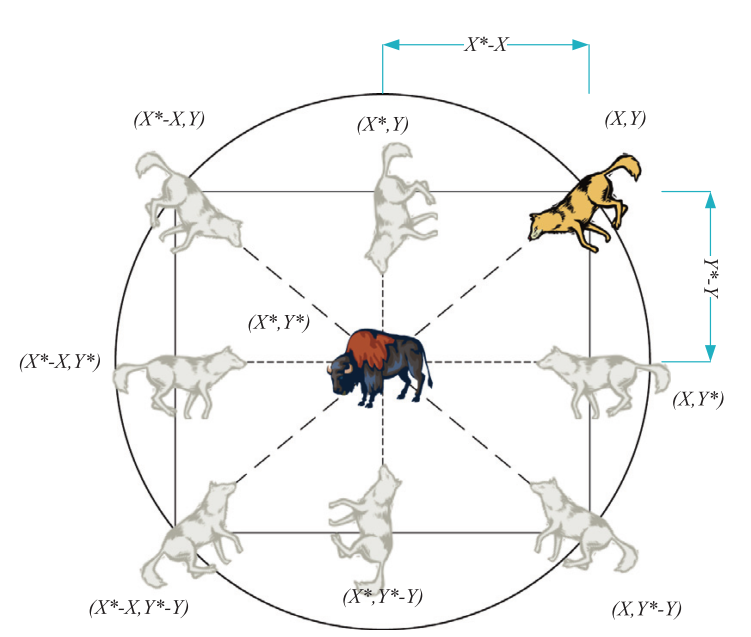
\includegraphics[width=\textwidth]{wolf_vector_positions.png}
  \caption{Príklad možného umiestnenia vlka v dvojrozmernom priestore na základe polohy koristi.}
	\source{Seeley, T. D.; Camazine, S.; Sneyd, J.: Collective decision-making in
					honey bees: how colonies choose among nectar sources. Behavioral
					Ecology and Sociobiology, ročník 28, č. 4, 1991: s. 277–290, ISSN
					1432-0762, doi:10.1007/BF00175101. URL http://dx.doi.org/10.1007/BF00175101}
  \label{fig-wolf-pos}
\end{figure}

\paragraph{Hľadanie koristi} je zabezpečené vektorom $\vec{A}$, ktorý mimo
intervalu [-1, 1] núti vlky divergovať od seba, čím je zdôraznená potreba
prehľadávať okolie a neskĺznuť do lokálneho minima. Náhodný vektor $\vec{C}$
simuluje prekážky v prírode, s ktorými sa vlk stretne pri hľadaní koristi.
V závislosti od vygenerovanej hodnoty, môže simulovať aj opačný prípad, ktorý
je pre vlka priaznivejší~\cite{Seeley1991}.

\paragraph{Lov} je vedený alfa vlkmi, beta a delta vlky sa tiež môžu na ňom
príležitostne podieľať. V prírode disponujú schopnosťou rozpoznať
umiestnenie koristi a obkľúčiť ju, avšak pri simulácií tohto správania, nemáme
vedomosť o presnej polohe koristi. Preto na základe prvých troch najlepších
riešení vypočítame predpokladanú polohu koristi, čím vznikne
vzorec~\ref{eq-prey-pos}. Kandidáti, vrátane omega vlkov, potom na základe
rovníc~\ref{eq-prey-x1},~\ref{eq-prey-x2}~a~\ref{eq-prey-x3} aktualizujú svoju
polohu~\cite{Seeley1991}.
\begin{equation}
  \vec{X}(t+1) = \frac{\vec{X_1} + \vec{X_2} + \vec{X_3}}{3}
  \label{eq-prey-pos}
\end{equation}

\paragraph{Útok} na korisť v matematickom modely dosiahneme približovaním sa ku
koristi, čiže znížením hodnoty $\vec{a}$. Tak dosiahneme aj zníženie hodnoty
$\vec{A}$ až bude jeho hodnota v intervale [-1, 1]. Potom ďalšia vypočítaná
hodnota pozície vlka sa bude nachádzať medzi jeho pôvodnou polohou a polohou
koristi. V prípade, že hodnota $\vec{A}$ sa nachádza mimo spomínaného
intervalu, vlk diverguje od koristi, čo nastáva vo fáze jej hľadania. Tým
je zabezpečené prehľadávanie priestoru agentami~\cite{Seeley1991}.

\paragraph{Princíp optimalizácie svorkou divých vlkov} môžeme znázorniť
v nasledujúcom pseudokóde~\cite{Seeley1991}
\begin{algorithm}[H]
  \caption{Pseudokód optimalizácie svorkou divých vlkov}
  \begin{algorithmic}[1]
    \State Náhodná inicializácia vlkov
    \State Inicializácia $a$, $A$ a $C$
    \State Vyhodnotenie fitness funkcie pre každého jedinca
    \State Priradenie do 3 najlepších riešení do $X_\alpha$, $X_\beta$ resp. $D_\delta$
    \State Opakuj kroky \ref{gwo-while} až \ref{gwo-iter} pokiaľ nebude prekročený maximálny počet iterácií \label{gwo-while}
    \State Aktualizovanie polohy na základe rovníc rovníc~\ref{eq-prey-x1},~\ref{eq-prey-x2}~a~\ref{eq-prey-x3}
    \State Aktualizovanie $a$, $A$ a $C$
    \State Vyhodnotenie fitness funkcie pre každého jedinca
    \State Aktualizovanie $X_\alpha$, $X_\beta$ a $D_\delta$
    \State Aktualizovanie počtu iterácií \label{gwo-iter}
    \State Vráť optimálne riešenie $X_\alpha$
  \end{algorithmic}
\end{algorithm}

%-------------------------------------------------------------------------------
%   Artifical bee colony
%-------------------------------------------------------------------------------

\subsubsection{Umelá kolónia včiel}
V literatúre označovaný ako ABC algoritmus (Artifical bee colony) je pomerne
nový medzi rojovými algoritmami. Princíp je založený na biologickom procese
správaní medonosných včiel pri hľadaní potravy. Každá včela pracujúca
v roji sa spolupodieľa na tvorbe celého systému na globálnej úrovni. Správanie
systému je určené lokálnym správaním, kde spolupráca a zladenie jedincov vedie
k štruktúrovanému kolaboračnému systému~\cite{Chavan2015}.

V algoritme, kolónia umelých včiel pozostáva z 3 skupín. Sú to včely
robotnice, diváčky a prieskúmníčky. Informácie o zdrojoch potravy si vymieňajú
tancovaním (waggle dance) na tzv. tanečnej ploche. Diváčky čakajúce na tanečnej
ploche sa rozhodujú, ktorý zdroj potravy si vyberú. Robotnice najskôr tieto
zdroje navštívia a prieskumníčky uskutočňujú náhodné prehľadávanie priestoru.
Pri aplikovaní ABC algoritmu, polovica včiel
predstavuje robotnice, druhá polovica diváčky. Počet robotníc zodpovedá počtu
zdrojov potravy v okolí úľu. Robotnica, ktorej zdroj je vyčerpaný inými
včelami sa stáva prieskumníčkou~\cite{Karaboga2007}.

Zväčšovaním množstva zdrojov potravy sa zväčšuje aj pravdepodobnosť vybratia
zdroja diváčkou. Vďaka tomu je zabezpečené, že tanec robotníc, ktoré navštívili
zdroje s najväčším množstvom nektáru, presvedčí najviac diváčok. Tie
na základe informácie o polohe zdroja nájdu v jeho okolí nový zdroj, z ktorého
budú zberať nektár. Po vyčerpaní nektáru je tento zdroj opustený a včela sa
presunie na zdroj, ktorý našli prieskumníčky~\cite{Karaboga2007}.

Pozícia zdrojov jedla je reprezentácia možného riešenia daného problému.
Množstvo nektáru je úmerné kvalite riešenia, ktoré je určené fitness funkciou.
Počet robotníc a diváčok je rovný počtu riešení v danej populácií, pričom každé
je reprezentovateľné ako D-dimenzionálny vektor. Hodnota $D$ môže
predstavovať počet optimalizačných parametrov~\cite{Karaboga2007}.

Včely majú riešenie uložené vo vlastnej pamäti, z ktorého modifikáciou vznikajú
nové, ktoré následné vyskúšajú. Ak je nové riešenie lepšie ako predchádzajúce,
včely si ho zapamätajú a predchádzajúce zabudnú. Inak si pamätajú staré. Keď
všetky robotnice skončia proces hľadania, zdieľajú informácie o zdrojoch
s diváčkami. Tie vyhodnotia zhromaždené informácie a vyberú zdroj s najlepším
riešením a jeho modifikovaním vytvoria nové, ktoré následne
skontrolujú~\cite{Karaboga2007}.

Diváčky vyberajú zdroj v závislosti od pravdepodobnosti zdroja $p_i$,
ktorú vypočítame ako
\begin{equation}
  p_i = \frac{fit_i}{\sum_{j = 1}^{n} fit_j}
  \label{eq-abc-prop}
\end{equation}
Vo vzorci \ref{eq-abc-prop} predstavuje $fit_i$ fitness funkciu, ktorá
ohodnocuje riešenie $i$. Týmto spôsobom si vymieňajú medzi sebou informácie
robotnice a diváčky~\cite{Karaboga2007}.

Algoritmus počíta nové riešenie na základe starého, čo matematicky zapíšeme ako
\begin{equation}
  v_{ij} = x_{ij} + \phi_{ij} (x_{ij} - x_{kj})
  \label{eq-abc-src}
\end{equation}
Ak si počet včiel definujeme ako $B$ potom na základe vzorca \ref{eq-abc-src}
platí $k \in {1, 2, ..., B}$ a $j \in {1, 2, ..., D}$. Indexy $k$ a $j$ sú
vybrané náhodne, ale $k$ musí byť rôzne od $i$. Hodnota $\phi_{ij}$ je
z intervalu [-1, 1] vyberaná náhodne. Je zrejmé, že čím bude menší rozdiel
medzi $(x_{ij}$ a $x_{kj})$, tým bude menší rozdiel aj medzi starým a novým
riešením~\cite{Karaboga2007}.

Algoritmus má 3 konfigurovateľné parametre a to: počet robotníc alebo diváčok,
ktorý je rovný počtu zdrojov jedla, limit, ktorý ohraničuje prehľadávaný
priestor a maximálny počet cyklov, ktorý sa vykoná ak sa skôr nenájde
optimálne riešenie~\cite{Karaboga2007}.

\paragraph{Princíp umelej kolónii včiel} znázorňuje nasledujúci
pseudokód~\cite{Karaboga2007}
\begin{algorithm}[H]
  \caption{Pseudokód umelej kolónie včiel}
  \begin{algorithmic}[1]
    \State Inicializácia včiel na náhodné zdroje potravy
    \State Opakuj kroky \ref{abc-while} až \ref{abc-end} pokiaľ nebude dosiahnutý cieľ \label{abc-while}
    \State Umiestnenie robotníc na zdroje potravy, ktoré boli nájdené
    \State Vyhodnotenie zdroja na základe množstva nektáru
    \State Umiestnenie diváčok na zdroje potravy na základe získaných informácií
    \State Vyhodnotenie, ktoré včely sa stanú prieskumníčkami
    \State Vyslanie prieskumníčok do prehľadávanie priestoru za účelom objavenia nových zdrojov potravy \label{abc-end}
    \State Vráť optimálne riešenie
  \end{algorithmic}
\end{algorithm}

%-------------------------------------------------------------------------------
%   Measurement of prediction accuracy
%-------------------------------------------------------------------------------

\subsection{Meranie presnosti predpovede}
Pre vyhodnotenie efektívnosti a presnosti modelov je potrebné merať ich
vlastnosti tak, aby sme ich vedeli medzi sebou porovnávať. V nasledujúcich
spôsoboch merania sú použité pojmy ako aktuálna hodnota $y_t$, predpovedaná
hodnota $f_t$ alebo chyba predpovede $e_t$ definovaná ako $e_t = y_t - f_t$.
Veľkosť testovacej množiny budeme označovať ako $n$~\cite{Agrawal2013}.

\subsubsection{Stredná chyba predpovede}
V literatúre označovaná ako MFE (mean forecast error). Matematickú funkciu
môžeme zapísať ako
\begin{equation}
  MFE = \frac{1}{n} \sum_{t=1}^{n} e_t
  \label{eq-mfe}
\end{equation}
Týmto spôsobom meriame priemernú odchýlku predpovedanej hodnoty od aktuálnej.
Zistíme tak smer chyby. Nevýhodou je, že kladné a záporné chyby sa vynulujú
a potom nie je možné zistiť presnú hodnotu chyby. Pri nameraní extrémnych chýb
nedochádza k žiadnej špeciálnej penalizácii. Taktiež hodnota chyby závisí od škály
meraní a môže byť ovplyvnená aj transformáciami dát. Dobré predpovede majú
hodnotu blízku 0~\cite{Agrawal2013}.

\subsubsection{Stredná absolútna chyba}
V literatúre označovaná ako MAE (mean absolute error). Patrí k jedným
z najpoužívanejších. Funkciu môžeme zapísať ako
\begin{equation}
  MAE = \frac{1}{n} \sum_{t=1}^{n} |e_t|
  \label{eq-mae}
\end{equation}
Týmto spôsobom meriame priemernú absolútnu odchýlku predpovedanej hodnoty od
aktuálnej. Zistíme tak celkový rozsah chyby, ktorá nastala počas predpovede.
Na rozdiel od merania chyby pomocou vzorca~\ref{eq-mfe} sa kladné a záporné
chyby nevynulujú, no ani napriek tomu nevieme určiť celkový smer chyby.
Na druhej strane tiež nenastáva žiadna penalizácia pri extrémnych chybách.
Hodnota chyby závisí od škály meraní a transformácií dát. Dobré predpovede majú
hodnotu čo najbližšiu 0~\cite{Agrawal2013, Gutierrez2015}.

\subsubsection{Stredná percentuálna chyba}
V literatúre označovaná ako MPE (mean percentage error). Matematicky môžeme
túto funkciu zapísať ako
\begin{equation}
  MPE = \frac{1}{n} \sum_{t=1}^{n} \frac{e_t}{y_t} \times 100
  \label{eq-mpe}
\end{equation}
Vlastnosti sú veľmi podobné ako pri MAPE v časti \ref{mape}. Chyba nám
poskytuje prehľad o priemernej chybe, ktorá sa vyskytla počas predpovede.
Naviac oproti MAPE získame prehľad o smere chyby, čo má však za následok, že
opačné znamienka sa vynulujú. O modely, ktorého chyba MPE sa blíži k 0,
nemôžeme s určitosťou tvrdiť, že funguje správne~\cite{Agrawal2013}.

\subsubsection{Stredná absolútna percentuálna chyba}
\label{mape}
V literatúre označovaná ako MAPE (mean absolute percentage error). Vzorec,
ktorým ju zapíšeme bude veľmi podobný vzorcu \ref{eq-mpe}
\begin{equation}
  MAPE = \frac{1}{n} \sum_{t=1}^{n} \Big|\frac{e_t}{y_t}\Big| \times 100
  \label{eq-mape}
\end{equation}
Pomocou tohto merania chyby získavame percentuálny prehľad o priemernej
absolútnej chybe, ktorá sa vyskytla počas predpovedi. Veľkosť chyby nezávisí od
škály merania, ale je závislá od transformácií dát. Tiež nie je možné zistiť
smer chyby a ani nenastáva žiadna penalizácia pri extrémnych
chybách~\cite{Agrawal2013}.

\subsubsection{Stredná štvorcová chyba}
V literatúre označovaná ako MSE (mean squarred error). Vzorcom ju zapíšeme ako
\begin{equation}
  MSE = \frac{1}{n} \sum_{t=1}^{n} e_t^2
  \label{eq-mse}
\end{equation}
Chyba meria priemernú štvorcovú odchýlku predpovedanej hodnoty. Opačné
znamienka sa neovplyvňujú. Neposkytuje nám pohľad na smer chyby. Zabezpečuje
penalizáciu extrémnych chýb. Zdôrazňuje fakt, že celková chyba je viac
ovplyvnená jednotlivými veľkými chybami ako viacerými malými. Nevýhodou je, že
chyba je veľmi citlivá na zmenu škály alebo transformáciu
dát~\cite{Agrawal2013}.

%-------------------------------------------------------------------------------
%   Analysis evaluation
%-------------------------------------------------------------------------------

\subsection{Zhodnotenie analýzy}
S rastúcim množstvom dát z rôznych zdrojov vzniká potreba predpovedať správanie
týchto veličín v budúcnosti. Existuje množstvo článkov, ktoré sa zaoberajú
týmto problémom. Neustále prinášajú a vylepšujú existujúce matematické modely,
ktoré sú schopné predpovedať budúce hodnoty meraných veličín. Výsledky nie sú
presné, ale chyba výpočtu je dostatočne nízka na to, aby sme takýto výsledok
mohli považovať za relevantný. Zvýšiť presnosť výsledkov je možné viacerými
metódami, či už kombináciou viacerých matematických modelov alebo ich
optimálnym nastavením. My sme sa v práci zamerali na hľadanie optimálneho
nastavenia používaných modelov.

Preskúmané predikčné modely potrebujú pre svoje správne fungovanie vstupné
parametre. Pomocou nich vieme ovplyvniť chybu predikcie. Problémom je nájdenie
takých parametrov, pre ktoré by bola chyba predikcie čo najmenšia. Hľadanie
najlepšieho riešenia by bolo časovo neprípustné, a preto budeme hľadať iba
optimálne riešenie, ktoré nám poskytne prijateľnú chybu predikcie. Je dôležité
poznamenať, že vstupné parametre, ktoré nájdu optimálnu predikciu závisia aj od
samotných dát. Ako bolo spomenuté v sekcii~\ref{time-series-analysis}, dáta
pozostávajú z viacerých zložiek a ich pomer sa môže líšiť pri rôznych
veličinách.

Na hľadanie optimálneho nastavenie predikčných algoritmov sme použili
prírodne inšpirované optimalizačné algoritmy. Ako ich názov napovedá, hľadanie
optimálneho riešenia sa vykonáva na základe správania sa nejakého živočíšneho
druhu alebo prírodného javu. Tieto algoritmy sa osvedčili ako efektívne a
rýchle riešenie problémov, ktorých prehľadávaný priestor riešení nie je možné
prehľadať celý. Algoritmy sa vyhýbajú spadnutiu do lokálnych miním a tak je
nájdené riešenie obvykle optimálne v globálnom rozsahu. A taktiež tieto algoritmy
poskytujú niekoľko konfiguračných parametrov ovplyvňujúce rýchlosť a presnosť
nájdeného riešenia. Avšak cieľom tejto práce je optimalizovať predikčné
a nie optimalizačné algoritmy a poskytnúť tak používateľovi univerzálne
a jednoduché riešenie predikčných problémov.

Dôležitou súčasťou predpovedí je vyhodnotenie ich úspešnosti porovnávaním
predpovedanej hodnoty s ich skutočnými nameranými hodnotami. Existuje množstvo
metód, ktorými vieme zmerať chybu predpovede. Niektoré nám poskytujú informáciu
o smere chyby, iné zohľadňujú extrémne chyby. Výsledky niektorých sa viažu na
škálu, v ktorej sa nachádzajú naše merania, iné sú nezávislé, merané v
percentách. Našim cieľom bolo poskytnúť používateľovi čo najviac informácií
o presnosti predpovede, a preto sú použité viaceré metódy merania chýb
predikcií.

%-------------------------------------------------------------------------------
%   Chapter 3 - Requirements specification
%-------------------------------------------------------------------------------

\newpage
\section{Špecifikácia požiadaviek}
\label{specification}
Cieľom práce je navrhnúť systém, ktorý umožní používateľovi nájsť optimálne
nastavenie vstupných parametrov predikčných metód. Používateľ bude mať
k dispozícií niekoľko predikčných a optimalizačných algoritmov, bude môcť
meniť ich konfiguračné parametre a vykonávať výpočty, vďaka ktorým zistí okrem
veľkosti predikčnej chyby aj optimálne nastavenie paramterov. Tieto výsledky
môže použiť vo vlastnej aplikácií alebo výskume. Predmetom optimalizácie budú
parametre predičkných metód, konfigurácia optimalizačných algoritmov je
ponechaná na používateľovi. Množinu dát si sám zvolí, aplikácia
je nezávislá na doméne, v ktorej boli dáta namerané. Ku každému z uvedených
parametrov bude poskytnuté vysvetlenie a opis zmeny správania na základe
ich zmeny. Presnosť predpovede bude určená pomocou používaných metrík na
meranie chyby predikcie. Keďže metrík je viacero, používateľ bude mať možnosť
si vybrať jednu z nich a tá bude následné použitá optimalizačných algoritmom.

Pri návrhu aplikácie boli použité dáta z inteligentných elektromeračov
používaných na Slovensku. Dostupné sú každých 15 minút z rôznych obcí. Keďže
budeme vždy predpovedať práve jednu veličinu práve jedného merača, každé
meranie potom bude jednoznačne identifikovateľné pomocou dátumu a času, kedy
bolo uskutočnené. Nameraná hodnota bude reprezentovaná reálnym číslom.
Našou úlohou nie je optimalizovať predpovede na základe faktorov, ktoré ich
ovplyvňujú a teda merania, ktoré majú k dispozícií aj hodnotu nejakej vysvetľujúcej
premennej budú spracovávané rovnakým spôsobom ako tie bez nej. Fungovanie
aplikácie nie je závislé na doméne, z ktorej dáta pochádzajú. Používateľ tak
môže optimalizovať predikčné parametre aj na základe iných dát ako z elektromeračov.

Používateľ si bude môcť vyberať z ponúknutých predikčných a optimalizačných
algoritmov. K dispozícii bude mať stochastické modely,
regresiu založenú na podporných vektoroch, rozhodovacie stromy a prírodne
inšpirované optimalizačné algoritmy ako umelú kolóniu včiel alebo optimaliziu
založenú na správaní roja častíc. Systém bude navrhnutý tak, aby pridanie
ďalších algoritmov nespôsobovalo zmeny v pôvodnej aplikácii a pozostávalo tak
iba z pridania implementácie algoritmov a prípadne zmeny konfigurácie.
Pripadá do úvahy, že samotný systém bude poskytovať rozhranie, ktoré
používateľovi umožní použiť vlastnú implementáciu iných algoritmov.

Optimalizačné algoritmy potrebujú mať určený definičný obor. Hodnoty
z neho používajú na nájdenie optimálneho riešenia, čo je v našom prípade
nájdenie kombinácie vstupných parametrov predikčných metód, ktorých výsledná
chyba je čo najmenšia. Z tohto dôvodu je dôležité myslieť pri návrhu aplikácie
na to, aby výstupom zvolených metód na meranie chyby boli nezáporné čísla.
V aplikácií sa budú nachádzať prednastavené definičné obory, ktoré bude môcť
používateľ v definovanom rozmedzí upravovať. Predídeme tak dlhým odozvám
systému pri zvolení veľkého definičného oboru a zároveň nevzniknú situácie,
kedy používateľ zvolí hodnotu, ktorá nebude patriť do definičného oboru
predikčnej metódy.

Systém bude implementovaný v jazyku R a webové používateľské rozhranie bude
vytvorené pomocou knižnice Shiny. Web aplikácie bude navrhnutý tak, aby
používateľovi poskytoval interaktívne rozhranie s predikčnými metódami.
Bude dostatočne robustný a intuitívny, aby s jeho používaním nemali problémy
ani tí menej skúsení. Zároveň bude skúsenému používateľovi poskytovať
modulárnosť, konfigurovateľnosť, ale hlavne rozhranie pre jednoduché pridávanie
ďalších algoritmov, ktoré si môže sám implementovať.

Spomenúté vlastnosti môžeme rozdeliť na funkcionálne a nefunkcionálne
nasledujúcimi odrážkami.

\noindent
\paragraph{Funkcionálne požiadavky:}
\begin{description}
  \item[$\bullet$ webová aplikácia] implementovaná pomocou jazyka R a knižnice Shiny
  \item[$\bullet$ vkladanie dát] používateľom v predefinovanom formáte
  \item[$\bullet$ výber predikčnej metódy] z implementovaných metód závisí od používateľovej voľby
  \item[$\bullet$ výber optimalizačnej metódy] ovyplvňuje rýchlosť a optimálnosť vypočítaného výsledku
  \item[$\bullet$ chyba predpovedi] je použítá pri optimaiizácií ako fitness funkcia
  \item[$\bullet$ vyhodnotenie výpočtu] zobrazením veľkosti chyby, nájdených optimálnych parametrov a vykreslením grafu
\end{description}

\noindent
\paragraph{Nefunkcionálne požiadavky:}
\begin{description}
  \item[$\bullet$ efektívnosť] implementácie je kľúčová pre zazpečenie rýchleho výpočtu výsledku
  \item[$\bullet$ jednoduchosť] použitia webovej aplikácie aj napriek množstvu parametrov, ktoré môže používateľ meniť
  \item[$\bullet$ modulárnosť] dovoľuje skúsenému používateľovi pridávať vlastné predikčné a optimalizačné algoritmy
  \item[$\bullet$ konfigurovateľnosť] aplikácie bude zabezpečená viacerými konfiguračnými súbormi
\end{description}

%-------------------------------------------------------------------------------
%   Chapter 4 -  Solution design
%-------------------------------------------------------------------------------

\newpage
\section{Návrh riešenia}
\label{solution-design}
Výsledná webová aplikácia bude používateľovi poskytovať možnosť zvoliť si
optimalizačný algoritmus, ktorým bude optimalizovať nastavenie predikčného
algortimu. Keďže každý predikčný algoritmus potrebuje pre správnu funkcionalitu
iné parametre s rôznymi hodnotami, je najskôr potrebné implementovať rozhranie,
ktoré zabezpečí správnu interakciu s optimalizačným algoritmom. Používateľ
preto bude vyberať iba z algoritmov, ktoré budú predom implementované alebo tak
sám urobí.

V práci som sa rozhodol zvoliť ako predikčné algoritmy metódu podporných
vektorov, autoregresívny integrovaný model kĺzavého priemeru a náhodné lesy.
Aplikácia je však navrhnutá genericky a pridanie ďalšieho algoritmu vyžaduje
minimálne úsilie. Kvôli malému počtu implementovaných optimalizačných
algoritmov v jazyku R som zvolil optimalizáciu rojom častíc a ABC
optimalizáciu. Používateľ bude môcť pomocou rozhrania určiť parametre pre tieto
algoritmy, ako napr. počet častí alebo cyklov.

%-------------------------------------------------------------------------------
%   Features of input data
%-------------------------------------------------------------------------------

\subsection{Vlastnosti vstupných dát}
Vstupné dáta, ktoré vkladá do aplikácie používateľ by mali byť vo formáte CSV,
teda súbor s tabuľkovými dátami, kde hodnoty v stĺpcoch sú oddelené čiarkami.
Súbor by mal pri tom obsahovať aspoň dva pomenované stĺpce, kde stĺpec ``timestamp''
obsahuje dátum a čas získania hodnoty, ktorá sa nachádza v stĺpci ``value''.
Hodnoty v ostatných stĺpcoch budú ignorované.
Zámerom bolo, aby zápis dátumu a času zodpovedal medzinárodnému štandardu
ISO 8601. Kvôli zložitosti čítania času v takomto formáte v použitom
implementačnom prostredí som zvolil vlastný formát dátumu, ktorý mu je veľmi
podobný. Formát dátumu je ``\%Y-\%m-\%d \%H:\%M:\%S'', podrobný rozbor sa
nachádza v tabuľke~\ref{tab-timestamp}. Z pohľadu návrhu aplikácie je potrebné,
aby vstupné dáta mali rovnaký počet meraní nameraných v jeden deň v celej
vstupnej množine. To znamená, že veľkosť periódy dát by mala byť rovnaká
a zároveň sa rovnala veľkosti periódy, ktorú zvolil používateľ vo webovej
aplikácii.

\begin{table}[ht]
  \centering
  \caption{Rozbor formátu dátumu a času.}
  \label{tab-timestamp}
  \begin{threeparttable}
    \begin{tabular}{|l|c|c|}
      \hline
      \textbf{Názov}  &   \textbf{Formátový reťazec}  &   \textbf{Hodnota}  \\ \hline
      Rok     & \%Y & 2013 \\ \hline
      Mesiac  & \%m & 07 \\ \hline
      Deň     & \%d & 10 \\ \hline
      Hodina  & \%H & 20 \\ \hline
      Minúta  & \%M & 15 \\ \hline
      Sekunda & \%S & 15 \\ \hline
    \end{tabular}
    \begin{tablenotes} \footnotesize
      \item $^{*}$ Dátum z tabuľky je ``2013-07-10 20:15:00''
    \end{tablenotes}
  \end{threeparttable}
\end{table}

Stĺpec s hodnotou obsahuje reálne číslo, ktoré reprezentuje veľkosť nameranej
veličiny, ktorú sa bude aplikácia snažiť predpovedať. Jednotky, v ktorých budú hodnoty
uvedené nie sú podstatné, výpočet je nezávislý na použitej škále. Obmedzenia
na tento stĺpec sú, aby skutočne obsahoval iba reálne číslo zodpovedajúce
nameranej hodnote a aby v rámci jedného súboru bola konzistentne použitá
rovnaká škála hodnôt. V stĺpci sa tak nesmie nachádzať názov či skratka
jednotky, v ktorej je hodnota nameraná.

V prípade, že pri vkladaní súboru aplikácia nenájde spomínané stĺpce, nedovolí
používateľovi spustiť výpočet. Pri návrhu aplikácie sa predpokladalo, že vstupné
dáta budú vždy pochádzať z jedného zariadenia a budú teda mať rovnakú časovú
zónu. Z tohto dôvodu stĺpec ``timestamp'' neobsahuje údaj o časovej zóne,
v ktorej bola hodnota nameraná. Dáta, ktoré som používal pri návrhu aplikácie
preto museli byť orezané tak, aby všetky dni mali rovnaký počet meraní alebo
čas musel byť prekonvertovaný do takej časovej zóny, ktorá by nespôsobovala
rôznu veľkosť periódy. Keďže množina dát, s ktorými som pracoval bola dostatočne
veľká zvolil som prvú možnosť.

Dáta by samozrejme nemali byť náhodné, ale malo by sa jednať o časový rad,
ktorý je možné dekomponovať na cyklickú, trendovú a náhodnú zložku. Niektoré
predikčné algoritmy priamo používajú dekompozíciu časových radov na
predpovedanie hodnôt. Jednotlivé záznamy o meraniach by mali za sebou
chronologicky nasledovať. V rámci jedného vstupného súboru musia mať dáta
všetky záznamy rovnakú periódu časového radu. Ak používateľ vo webovom rozhraní
zvolí, že vložené dáta majú periódu napr. 96 meraní za deň, potom aj aplikácia
bude očakávať zvolenú veľkosť periódy. Ak pri overovaní dojde k zlyhanie
aplikácie ohlási chybu.

%-------------------------------------------------------------------------------
%   Used prediction algorithms
%-------------------------------------------------------------------------------

\subsection{Použité predikčné metódy}
Z pohľadu návrhu aplikácie nás budú pre každú predikčnú metódu zaujímať najmä
vstupné parametre, ktoré budeme optimalizovať a transformácie, ktoré je
potrebné nad vstupnými dátami vykonať. Takéto delenie je dôležité aj kvôli
organizácií programu pri implementácií, keďže úprava dát sa vykoná iba raz,
zatiaľ čo vstupné paramete sa budú meniť neustále. Výstupom výpočtu predpovede
bude samotná predpoveď alebo veľkosť chyby dosiahnutá pri nej dosiahnutá.

\subsubsection{Regresia založená na podporných vektoroch}
Parametre, ktoré budeme optimalizovať budú $C$ a $\varepsilon$, ktoré môžu
nadobúdať iba kladné hodnoty. Hodnota parametru $C$ reprezentuje cenu za
prekročenie hranice, ktorú sme definovali. Hranicu si označíme ako $\varepsilon$.
% TODO je epsilon táto hranica
To znamená, že pri veľmi nízkej hodnote sa výsledná predikcia podobá na
konštantnú funkciu. Pri veľmi vysokej hodnote môže dôjsť k pretrénovaniu modelu
a zvýšeniu výslednej chyby na množine testovacích dát. Hodnota parametru
$\varepsilon$ je hodnota použitá v nesenzitívnej stratovej funkcii, ktorá sa
% TODO epsilon in the insensitive-loss function
používa pre regresiu. Zvyšovaním tejto hodnoty sa funkcia reprezentujúca
predpoveď postupne vyhladzuje, až sa bude podobať na konštantú funkciu.

Vstupné dáta je potrebné tranformovať na 2 matice, jednu trénovaciu maticu
a jednu testovaciu maticu. Trénovacia matica obsahuje stĺpec s hodnotami,
ktoré boli v daných časoch namerané, testovacia má tento stĺpec prázdny,
predpovedané hodnoty doplní algoritmus. Počet ďalších stĺpcov sa môže líšiť
v závislosti od veľkosti zvolenej periódy. Ak si označíme počet meraní za deň
ako $n$, potom stĺpce $C_1$ až $C_n$ budú obsahovať hodnotu 1 práva vtedy,
keď poradie merania v dni bude totožné s poradím stĺpca. Rovnakým postupom
pridáme ešte ďalších 7 stĺpcov, ktoré budú predstavovať poradie dňa v týždni.
Pre iné stĺpce $C_1$ až $C_7$ bude potom platiť, že napr. v prvom stĺpci bude
priradená hodnota 1 tým záznamom, ktoré boli namerané v pondelok. Zvyšok matíc
bude doplnení nulami.

\subsubsection{Autoregresívny integrovaný model kĺzavého priemeru}
Parametre stochastického modelu ARIMA sú v literatúre označované ako $p$, $d$
a $q$. Z kapitoly~\ref{stochastic} vieme, že model ARIMA je generalizáciou
modelu ARMA, ktorý vznikol kombináciou autoregresívneho modelu a modelu
kĺzavých priemerov. Vstupné parametre sú nezáporné celé čísle, kde $p$ a $q$
predstavuje rad modelu a $d$ zodpovedá stupňu derivovania. Pri veľkom počte
derivovaní sa funkcia predpovednej hodnoty podobá linárnej funkcii.
% TODO Ostatné parametre netuším ako prispievajú k dielu, okrem toho, že im to trvá

Príprava vstupných dát je veľmi jednoduchá. Keďže model pracuje priamo
s časovými radmi a vstupné dáta sú časový rad, jedinou úpravou je rozdelenie dát
na trénovaciu a testovaciu množinu a určenie veľkosti periódy, ktorú zadáva
používateľ.

\subsubsection{Náhodné lesy}
Vstupné parametre, ktoré sa budeme snažiť v aplikácií optimalizovať bude počet
stromov a minimálna veľkosť uzlu v stromoch. Je zrejmé, že číslo definujúce
počet stromov bude musieť byť kladné a celé, zatiaľ čo veľkosť uzlu môže byť
definovaná ako ľubovoľné nezáporné číslo. Pri zvyšovaní počtu stromov, ktoré
budú vytvorené sa funkcia predpovedanej hodnoty javí, akoby každé pridanie stromu
poskytovalo funkcii ďalšiu možnosť zmeny smeru. Funkcia tak pri malom počte
stromov vyzerá kostrbato a náhodne, zväčšovaním počtu sa extrémy vyhladzujú a
predpovedané hodnoty postupne konvergujú do funkcie, ktorá je obrysmi podobná
funkcii reálnych dát. Zväčšovaním uzlov sa funkcia predikovaných hodnôt
postupne vyhladzuje, až nakoniec opisuje konštantnú funkciu.

Rovnako ako model ARIMA tak aj náhodné lesy pracujú priamo s časovými radmi.
Je však potrebné pridať k dátam informáciu o tom, kedy boli namerané. Zároveň
by táto funkcia mala byť spojitá. To najjednoduchšie dosiahneme tak, že z dátumu
extrahujeme poradie dňa v týždni a z časovej zložky zasa poradie merania v dni.
Funkcie zatiaľ nie sú spojité, a preto na ne aplikujeme transformáciu popísanú
vo vzorci~\ref{eq-rf-prepare}~\cite{Laurinec2017}
\begin{equation}
  \frac{sin(2\Pi \frac{\text{poradie merania}}{\text{veľkosť periódy}}) + 1}{2} \text{  resp.  } \frac{cos(2\Pi \frac{\text{poradie merania}}{\text{veľkosť periódy}}) + 1}{2}
  \label{eq-rf-prepare}
\end{equation}
a goniometrické funkcie sínus a kosínus. Výsledné funkcie sú spojité a svojou
harmonickosťou opisujú vlastnosti dát skryté v dátume a čase. Priebeh 4 pomocných
funkcií je znázornení na obrázku~\ref{fig-rf-prepare}.

\begin{figure}[ht]
  \centering
  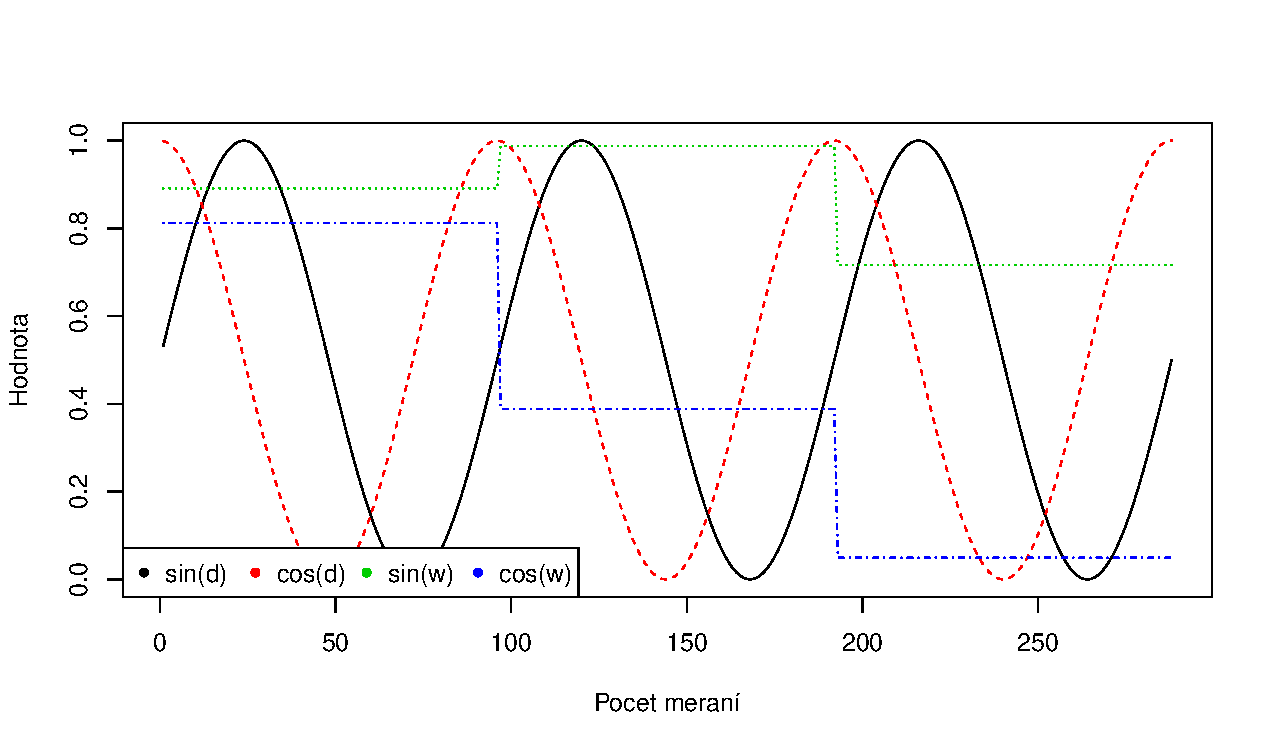
\includegraphics[width=\textwidth]{random_forest_preparation.pdf}
  \caption{Ukážka transformácií dátumu a času pri predikcii náhodnými lesmi.}
  \label{fig-rf-prepare}
\end{figure}

%-------------------------------------------------------------------------------
%   Used optimization algorithms
%-------------------------------------------------------------------------------

\subsection{Použité optimalizačné metódy}
Aplikácia bude používateľovi poskytovať rozhranie na nastavenie vstupných
parametrov predikčných metód a taktiež nastavanie rozsahu hodnôt, ktoré majú
tieto metódy použiť pri optimalizovaní. Výsledkom výpočtu bude porovnanie
reálnych a predpovedaných dát v podobe grafu a veľkosti výslednej chyby.
Taktiež budú používateľovi zobrazené optimálne parametre pre zvolenú predikčnú
metódu. Každá kombinácia parametrov vystupuje v optimalizačnom algoritme ako
agent, ktorého úlohou je dosiahnuť, čo najnižšiu hodnotu fitness funkcie.
V závisloti od použitého algoritmu a získaných vedomostí sa v nasledujúcich
cykloch menia hodnoty reprezentujúce agenta. Hodnoty parametrov môžu byť
ovplyvňované aj voľbou funkcie na meranie chyby, ktorá plní úlohu fitness
funkcie pre optimalizačné algortimy.

Pri návrhu aplikácie je dôležité najmä správne definovať rozhranie medzi
predikčnými a optimalizačné metódami. Je nemysliteľné, aby pri pridávaní
ďalších algoritmov bolo potrebné upravovať už používané algoritmy, najmä kvôli
množstvu kombinácií, ktoré môže vzniknúť. Našťastie každého agenta definujeme
práve hodnotami, ktoré vstupujú do predikčného algoritmu. Na výstupe očakáva
optimalizačná metóda hodnotu fitness funkcie, ktorá určuje ďalšie smerovanie
agentov. Tento proces sa opakuje až pokiaľ nebude dosiahnutá ukončovacia
podmienka. V použitých algoritmoch to je maximálny počet iterácií algortimu.
Túto hodnotu môže používateľ nastaviť v aplikácií v definovanom rozsahu.

\subsubsection{Optimalizácia rojom častíc}
Používateľ bude mať možnosť v aplikácií zvoliť počet častíc, ktoré budú
použité na optimalizovanie problému. Pod každou časticou si môžeme predstaviť
agenta, ktorý bude nositeľom informácie o okolitom prostredí a o hodnotách,
ktoré ho viedli k aktuálnemu riešeniu. Pre každý optimalizovaný parameter je
potrebné definovať rozsah hodnôt, ktoré môže používateľ v aplikácií nastaviť.
Je dôležité poznamenať, že okrem hraníc rozsahu nás zaujímajú aj samotné
hodnoty, ktoré bude algoritmus používať na optimalizáciu. Je zrejmé, že
používať desatinné čísla pre parameter označujúci napr. počet stromov nie je
logické a aplikácia by mala byť schopná sa s tým vysporiadať.

V prostredí jazyka R sú k dispozícií 2 rôzne knižnice implementujúce
optimalizáciu rojom častíc. V aplikácií sa budú pre porovnanie použité obidve
implementácie.

\subsubsection{Umelá kolónia včiel}
Rovnako ako pri optimalizácii rojom častíc tak aj pri tomto algoritme bude mať
používateľ možnosť zvoliť rozsah hodnôt, ktoré budú použité na optimalizovanie.
Opäť bude dôležité vysporiadať sa s desatinými číslami. Používateľ bude môcť
navyše nastavovať parametre ABC algoritmu ako je počet zdrojov potravy alebo
limit pre daný zdroj. Pod limitom môžeme rozumieť počet iterácií cyklu, počas
ktorého sa daný zdroj potravy nezlepšil. Týmto parametrom môžeme výrazne
urýchliť nájdenie optimálneho riešenia, na druhej strane môže nastať situácia,
kedy by sme rýchlym opustením zdroja potravy mohli stratiť lepšie riešenie.
Zvyšovaním počtu zdrojov potravy sa zvyšuje aj čas výpočtu, ale zároveň bude
nájdené optimálnejšie riešenie.

%-------------------------------------------------------------------------------
%   Chapter 5 - Implementation
%-------------------------------------------------------------------------------

\newpage
\section{Implementácia}
\label{implementation}
Webová aplikácia je implementovaná v jazyku R verzie 3.4.0. Pri implementácií
som používal developerské prostredie RStudio verzia 1.0.143. Webové rozhranie je
vytvorené pomocou knižnice ``shiny''. Konfigurácia aplikácie je zabezpečená
knižnicou ``config'', informácie o ďalších použitých knižniciach a ich verziách
sa nachádzajú v tabuľke~\ref{tab-libraries}. Nasledujúce podkapitoly obsahujú
popis použitých transformáciami nad dátami, popis organizácie zdrojového kódu
do funkcií a súborov, úpravu konfigurácie, ale aj postupy na pridanie ďalších
predikčných a optimailzačných algoritmov.

\begin{table}[ht]
  \centering
  \caption{Použité knižnice jazyka R.}
  \label{tab-libraries}
  \begin{tabular}{|l|l|}
    \hline
    \textbf{Názov}  &   \textbf{Použitá verzia}  \\ \hline
    ABCoptim        &   0.14.0  \\ \hline
    config          &   0.2     \\ \hline
    forecast        &   8.0     \\ \hline
    kernlab         &   0.9-25  \\ \hline
    pso             &   1.0.3   \\ \hline
    psoptim         &   1.0     \\ \hline
    randomForest    &   4.6-12  \\ \hline
    shiny           &   1.0.2   \\ \hline
    shinyjs         &   0.9     \\ \hline
  \end{tabular}
\end{table}

%-------------------------------------------------------------------------------
%   Cleaning input data
%-------------------------------------------------------------------------------

\subsection{Úprava vstupných dát}
Počas návrhu aplikácie bolo k dispozícií viacero datasetov, ktoré sme mohli
použiť. Keďže je fungovanie aplikácie nezávislé na zvolenej doméne a nevzniká
potreba trénovať model na veľkom množstve dát, jediným kritériom na vstupné
dáta je, aby mali vlasnosti časových radov. Použité dáta pochádzajú
z inteligentných elektromeračov nachádzajúcich sa na Slovensku. Veličina, ktorú
sme predpovedali je odber elektrickej energie. Dáta sú k dispozícií každých
15 minút a celý dataset obsahuje merania z obdobia takmer 2 rokov. Formát
dát je nasledovný:

\begin{lstlisting}{R}
  DATUM,CAS,Suma_odbery
  01/07/2013,-105,1979.647687
  01/07/2013,-90,1866.069666
  01/07/2013,-75,1657.762122
  01/07/2013,-60,1646.840106
  01/07/2013,-45,1654.063798
  01/07/2013,-30,1719.126487
  01/07/2013,-15,1725.385136
  01/07/2013,0,1702.126518
  01/07/2013,15,1653.233316
  01/07/2013,30,1601.772426
  01/07/2013,45,1577.106243
  01/07/2013,60,1553.637892
  01/07/2013,75,1557.940842
  01/07/2013,90,1523.56265
\end{lstlisting}

Môžeme si všimnúť, že vstupný CSV súbor pozostáva z 3 stĺpcov ``DATUM'', ``CAS''
a ``\text{Suma\_odbery}''. Hodnoty času pritom nezodpovedajú formátu, na ktorý sme
bežne zvyknutý, hlavne preto, že sa jedná o jedno celé číslo, ktoré nadobúda aj
záporné hodnoty. Je to z dôvodu, že toto číslo označuje poradie merania v dni
v minútach v časovej zóne UTC, čiže záporné hodnoty tohto stĺpca označujú prvé
hodiny v dni. Pri letnom čase sú to dve hodiny a pri zimnom iba jedna. Ako bolo
spomenuté v kapitole~\ref{solution-design}, aplikácia nebude závislá od domény,
časovej zóny alebo pomocných premenných, no zároveň je potrebné zachovať
konzistentnú veľkosť periódy naprieč celým datasetom. Z toho dôvodu sa nám
naskytujú dva spôsoby, ktorými môžeme upraviť dátum a čas do požadovaného
formátu.

Prvým je odstránenie nadbytočnej hodiny pri prechode na zimný čas,
pridanie chýbajúcej hodiny pri prechode na letný čas (napr. opakovaním hodnôt
z predchádzajúcej hodiny) a následne prekonvertovať stĺpec ``CAS'' do formátu
``\%H:\%M:\%S'', s ktorým už ďalej vieme bez problémov pracovať. Druhým
jednoduchším spôsobom je obmedziť používanie aplikácie na dáta s veľkosťou
rádovo v týždňoch. Optimalizácia parametrov pri väčších dátach je aj tak veľmi
časovo náročná. Potom môžeme záporné hodnoty presunúť do predchádzajúceho dňa
a následne ich konvertovať spolu s dátumom do požadovaného formátu. Týmto
spôsobom stratíme iba jeden deň na začiatku a na konci časového radu. Cenu za
to je posunutie sledovanej veličiny spolu s posunutím času. Na výsledných dátach
sa to prejaví tak, že vzory, ktoré si môžeme všimnúť v dátach z letného času,
budú v zimnom čase o hodinu posunuté. Vstupná množina dát však nikdy nebude
väčšia ako pár mesiacov, a tak nie je problém vyhnúť sa dvom dátumom v roku.
Navyše tieto dáta boli použité iba pri návrhu a používateľ bude môcť použiť
dáta, ktoré sám uzná za vhodné. Výsledný formát dát je potom nasledovný:

\begin{lstlisting}{R}
  timestamp,value
  2013-07-01 00:00:00,1702.126518
  2013-07-01 00:15:00,1653.233316
  2013-07-01 00:30:00,1601.772426
  2013-07-01 00:45:00,1577.106243
  2013-07-01 01:00:00,1553.637892
  2013-07-01 01:15:00,1557.940842
  2013-07-01 01:30:00,1523.56265
\end{lstlisting}

Dáta v takomto formáte sú vhodné na spracovanie, avšak nie je možné ich priamo
použiť predikčnými algoritmami. Každý z nich očakáva, že pracuje s dátami
v rôznych dátových štruktúrach s rôznymi vysvetľujúcimi premennými. Aj keď bolo
spomenuté, že aplikácia ich nebude používať v prípade, že vstupné dáta obsahujú
viacero stĺpcov, v tomto prípade sa jedná o dekomponovanie zložiek časového radu
a transformovanie datúmu a času tak, ako to požaduje konkrétny algortimus.

Ako už bolo spomenuté SVR požaduje trénovacie aj testovacie dáta v štruktúre
matici, ktorá bude až na stĺpec s nameranou alebo predpovedanou hodnotou
obsahovať iba hodnoty 0 a 1. Po vytvorení matici, ktorá obsahuje iba 0, sa
postupne na ňu aplikujú metódy ``svr.setOnesForTimestamp'' a ``svr.setOnesForDayOfWeek'',
ktoré priradia hodnotu 1 pre stĺpec reprezentujúci poradie merania v dni a
rovnako aj pre stĺpec reprezentujúci poradie dňa v týždni, kedy bolo meranie
uskutočnené. Poslednou úpravou je pridanie stĺpca s nameranými hodnotami pre
trénovaciu maticu a prázdneho stĺpca pre testovaciu maticu. Implementácia
spomínaných funkcií je:

\begin{lstlisting}[language=R]
  svr.setOnesForTimestamp <- function(matrixM, dates, recordsCount, measurementsPerDay) {
    for (i in 1:recordsCount) {
      matrixM[i, svr.orderOfTimestamp(dates[i], measurementsPerDay) + 1] <- 1
    }
    return(matrixM)
  }


  svr.setOnesForDayOfWeek <- function(matrixM, dates, recordsCount, measurementsPerDay) {
    for (i in 1:recordsCount) {
      matrixM[i, measurementsPerDay + svr.nthInWeek(dates[i])] <- 1
    }
    return(matrixM)
  }
\end{lstlisting}

Pri opužití modelu ARIMA je transformácia vstupných dát jednoduchá. Model
dáta v štruktúre časového radu, v ktorej už samotné dáta sú. Príprava dát potom
spočíva iba v rozdelení množiny na časti požadované používateľom. Implementácia
je nasledovná:

\begin{lstlisting}[language=R]
  trainingTS <- ts(preparedData$trainingData$value, frequency = preparedData$measurementsPerDay)
  testingTS <- ts(preparedData$testingData$value, frequency = preparedData$measurementsPerDay)
\end{lstlisting}

V prípade transformácie dát pre náhodné lesy, by sme mohli hovoriť o kombinácii
predchádzajúcih dátových štruktúru s miernym vylepšením. Pri SVR vzniká matica
s veľkosťou desiatkami stĺpcov a stovkami riadkov, ktoré v každom riadku
obsahujú práve dve hodnoty 1, zvyšok sú samé 0. Dáta v takomto formáte je
zložité nejako graficky znázorniť a pritom sa jedná iba o 2 pílovité funkcie,
rastúce rozdieľnou rýchlosťou. Toto správanie by sme vedeli zachytiť aj dvoma
číslami, ktoré by reprezentovali rovnaké funkcie. Ak by sme však chceli získať
spojité funkcie, tak ako to požaduje implementácia náhodných lesov, je potrebné
aplikovať na dáta mapovanie znázornené obrázkom~\ref{fig-rf-prepare}. Harmonické
funkcie potom opisujú pozíciu merania v dni a týždni, čo implementujeme
nasledujúcimi funkciami:

\begin{lstlisting}[language=R]
  rf.setSinForDay <- function(dates, frequencyF) {
    return((sin(2 * pi * rf.nthInDay(dates, frequencyF) / frequencyF) + 1) / 2)
  }

  rf.setCosForDay <- function(dates, frequencyF) {
    return((cos(2 * pi * rf.nthInDay(dates, frequencyF) / frequencyF) + 1) / 2)
  }

  rf.setSinForWeek <- function(dates, frequencyF) {
    return((sin(2 * pi * rf.nthInWeek(dates, frequencyF) / frequencyF) + 1) / 2)
  }

  rf.setCosForWeek <- function(dates, frequencyF) {
    return((cos(2 * pi * rf.nthInWeek(dates, frequencyF) / frequencyF) + 1) / 2)
  }
\end{lstlisting}

%-------------------------------------------------------------------------------
%   Application architecture
%-------------------------------------------------------------------------------

\subsection{Architektúra aplikácie}
Pri vytváraní webovej aplikácie pomocou knižnice Shiny, sa program rozdeľuje na
časť webového rozhrania a serverovú časť. Tie sa pri jednoduchých aplikáciách
môžu nachádzať v jednom súbore, ja som ich podľa odporúčaní dokumentácie
rozdelil do súborov ``ui.R'' a ``server.R'' pre webové rozhranie serverovú
logiku. Konfiguračné súbory pomocou, ktorých sa do aplikácie jednoducho
pridávajú ďalšie algortimy sa nachádzajú v adresári ``conf''. Zdrojové kódy,
ktoré zabezpečujú úpravu dát a výpočet sa nachádzajú v adresári ``src''.
Keď sa podrobnejšie pozrieme na obsah tohto adresára zistíme, súbory sú
očíslované prefixom, ktorý zodpovedá logickému poradiu ich používania, ale
zároveň sú v tomto poradí aj importované pri spustení Shiny servera.

Predikčné algoritmy sú implementované v súboroch s prefixami ``01'' a ``03'',
za čím nasleduje skátený názov implementované algoritmu. Rozdeleným
implementácie do dvoch súborov sa oddelí príprava dát na výpočet od samotného
výpočtu. Názvy funkcií sú potom pomocou konfiguračného súboru namapované na
jednotlivé grafické komponenty vo webovom rozhraní. Názov funkcie má vždy ako
prefix skrátený názov algortimu, ktorý ho používa. Podobná konvencia je
dodržaná aj pri optimalizačných algoritmoch, s tým že prefix súborov je ``04''.
Volanie optimalizačných algoritmov zväčša pozostáva z jedného volania funkcie,
a preto nevzniká potreba delenia na viacero súborov. Načítanie dát zo súboru
a rôzne fitness funkcie sa nachádzajú v osobitnom súbore.

Aplikácia je navrhnutá tak, aby pridávanie ďalších algoritmov vyžadovalo, čo
najmenšie úsilie. Kvôli tomu sú grafické komponenty vykresľované zo súboru
``server.R'' a ``ui.R'' ako je to pri stránkach so statickým, prípadne
jednoducho dynamickým rozložením komponentov. Vykresľované sú na základe obsahu
konfiguračného súboru ``conf/server-config.yml'', ktorý v sebe obsahuje
mapovanie na použité metódy a na základe vstupov z grafického rozhrania, kde si
používateľ volí používané algoritmy. V závislosti od toho sa mení počet
zobrazovaných komponentov, ich obsah a význam. Komponenty vykresľované serverom,
by sme mohli rozdeliť na parametre optimalizačných metód a rozsahy
prehľadávania riešenie pre predikčné algoritmy.

%-------------------------------------------------------------------------------
%   Using Shiny library
%-------------------------------------------------------------------------------

\subsection{Použitie knižnice Shiny}
Webová aplikácia, s ktorou prichádza používateľ do styku je vytvorená pomocou
knižnice Shiny v jazyku R. Zdrojový kód býva obvykle organizovaný do súborov
``ui.R'' pre grafické komponenty a ``server.R'' pre logiku skrytú za nimi.
Zároveň je možné vykreslovať jednotlivé komponenty aj zo serverovej časti
aplikácie na predefinované miesto v ``ui.R''. Takéto použite má zmysel
v prípade, že zobrazované komponenty sa budú dynamicky pridávať a odoberať
v závislosti od zvolených možností. Tento príklad presne zodpovedá problému,
s ktorým sme sa stretli pri implementácií aplikácie. Zobrazovanie jednotlivých
parametrov závisí od predom zvolených metód. Navyše kvôli zachovaniu
konfigurovateľnosti je potrebné vlastnosti komponentov čítať z konfiguračného
súboru, čím strácame možnosť sa na ne jednoducho odkazovať. Zobrazovanie
komponentov priamo z ``server.R'' povolíme volaním funkcie
``uiOutput("predictionParameters")'' v ``ui.R''. Následne je potrebné priradiť
komponenty do premennej ``output\$predictionParameters'' v serverovej časti.
To zabezpečíme nasledujúcim zdrojovým kódom:

\begin{lstlisting}[language=R]
output$predictionParameters <- renderUI({ $ % TODO remove
  numberOfParameters <- length(server.properties$predictionAlgorithms[[as.numeric(input$predictionAlgorithms)]]$predictionParameters)
  fluidRow(
    lapply(1:numberOfParameters, function(i) {
      column(5,
       numericInput(server.properties$predictionAlgorithms[[as.numeric(input$predictionAlgorithms)]]$predictionParameters[[i]]$id,
        label = server.properties$predictionAlgorithms[[as.numeric(input$predictionAlgorithms)]]$predictionParameters[[i]]$label,
        value = server.properties$predictionAlgorithms[[as.numeric(input$predictionAlgorithms)]]$predictionParameters[[i]]$value,
        min = server.properties$predictionAlgorithms[[as.numeric(input$predictionAlgorithms)]]$predictionParameters[[i]]$min,
        max = server.properties$predictionAlgorithms[[as.numeric(input$predictionAlgorithms)]]$predictionParameters[[i]]$max,
        step = server.properties$predictionAlgorithms[[as.numeric(input$predictionAlgorithms)]]$predictionParameters[[i]]$step
       )
      )
    })
  )
}) $ % TODO remove
\end{lstlisting}

\begin{description}
  \item[$\bullet$ numberOfParameters] počet parametrov zvoleného predikčného algoritmu
  \item[$\bullet$ as.numeric(input\$predictionAlgorithms)] index zvoleného predikčného algoritmu pomocou, ktoré sa pristupuje do poľa algoritmov v konfiguračnom súbore
  \item[$\bullet$ server.properties\$predictionAlgorithms] pole predikčných algoritmov v konfiguračnom súbore
  \item[$\bullet$ lapply(1:numberOfParameters, function(i)] vytvorenie objektov typu ``column'' v cykle
  \item[$\bullet$ predictionParameters[[ i \textbf{]]} ] pristupovanie k jednotlivým parametrom nachádzajúcich sa v konfiguračnom súbore
\end{description}

Po vykreslení komponentov vzniká nový problém, ktorým je získanie hodnôt, ktoré
nastavil používateľ. Keďže nikdy nie sú vykreslené všetky komponenty a každý
z nich má iný identifikátor, museli by sme sa pri dotazovaní sa najprv uistiť,
či daný komponent existuje. To vy nebolo najvhodnejšie riešenie, keďže zároveň
by sme dosiahli aj množstvo duplicitných častí kódu a znížila by sa udržatelnosť
a čitetaľnosť. Ak by sme problém riešili rovnakými identifikátormi stále by to
neriešlo rôzne počty parametrov. Jediným rozumným riešením je opäť použiť
odkazovanie na hodnoty v konfiguračnom súbore, čo je zabezpečené funkciou
``setOptimizationParameters''. Kľúčovými časťami kódu je cyklus:

\begin{lstlisting}[language=R]
for (i in 1:predictParamsCount) {
  value <- eval(parse(text = paste("input", "$", predictParams[[i]]$id, sep = "")))

  if (grepl("^min", predictParams[[i]]$id)) {
    lows <- c(lows, value)
  }
  else if (grepl("^max", predictParams[[i]]$id)) {
    highs <- c(highs, value)
  }
}
\end{lstlisting}

\begin{description}
  \item[$\bullet$ predictParamsCount] počet parametrov zvoleného predikčného algoritmu
  \item[$\bullet$ predictParams] pole parametrov predikčného algoritmu
  \item[$\bullet$ value] hodnota, ktorá zadal používateľ, vzniká evaluovaním reťazca, ktorý spája používanú syntax a identifikátor komponentu z konfiguračného súboru
  \item[$\bullet$ if] vzhľadom na to, že pri optimalizácií vždy určujeme rozsah použitých hodnôt, môžeme ich identifikovať prefixom ``min'' a ``max'' a oddeliť ich od seba
\end{description}

%-------------------------------------------------------------------------------
%   Application configuration
%-------------------------------------------------------------------------------

\subsection{Konfigurácia aplikácie}
Aplikácia je ľahko konfigurovateľná a rozšíriteľná aj vďaka konfiguračným
súborom nachádzajúcich sa v adresári ``conf'', ale aj súboru ``global.R'',
ktorý sa automaticky importuje pri spustený Shiny servera. Obsahuje informácie
o cestách k súborom, ktoré aplikácia potrebuje pre správne fungovanie. Pri
použití aplikácie na inom operačnom systéme ako Linux, prípade s iným
rozmiestneným súborov, je možné v tomto súbore jednoducho zmeniť prednastavené
cesty.

Spomínaný konfiguračný adresár obsahuje ďalšie 3 súbory. Najdôležitejším je
``server-config.yml'' a možno ho logicky rozdeliť na 3 časti a to predikčné
algortimy, optimalizačné algoritmy a fitness funkcie. Každý z predikčných
algoritmov obsahuje názvy parametrov, ktoré budú optimalizované, názvy funkcií,
ktoré na to budú použité a názvy, ktoré budú zobrazované používateľovi pri
používaní aplikácie. Parametre v sebe zahŕňajú aj informáciu o minimálnych,
maximálnych a prednastavených hodnotách.

Ďalším konfiguračným súborom je ``ui-config.yml'', ktorý obsahuje väčšinou
texty a názvy jednotlivých komponentov, no nájdu sa tu aj hodnoty argumentov
pre komponenty, ktoré sa počas behu aplikácie nemenia. Takto je zmena jazyku
aplikácie veľmi jednoduchá a a vykonané zmeny by sa týkali iba týchto dvoch
súborov. Posledným konfiguračným súborom je ``app-config.yml'', kde sú
umiestnené hodnoty, ktoré sa netýkajú webovej aplikácie, ale samotných
algoritmov. Veľa z nich poskytuje väčšiu funkcionalitu ako sme reálne použili.
To vieme ovplyvniť pri volaní funkcie napr. nastavením príznaku alebo
konkrétnou hodnotou vymenovaného typu. Konkrétnym príkladom je predpovedanie
pomocou SVR, ktorý sa bežne používa na klasifikačné problémy ako SVM. V súbore
sa potom nachádza vymenovaný typ označujúci použitie regresie a nie klasifikácie.

%-------------------------------------------------------------------------------
%   Procedure for adding prediction algorithm
%-------------------------------------------------------------------------------

\subsection{Postup pridávania predikčných algoritmov}
Najdôležitejšou časťou pridania ďalšieho algoritmu je implementovanie 3 funkcií,
na ktoré sa neskôr budeme odkazovať z webového rozhrania. Prvá funkcia,
v konfiguračnom súbore označovaná ako ``prepareFn'', bude na vstupe očakávať
výsledok načítania súboru, čiže zoznam s dátami z trénovacej a testovacej
množine so stĺpcami ``timestamp'' a ``value'' a počet meraní za deň. Výstupom
funkcie je opäť zoznam, obsahujúci pripravené dátové štruktúry pre trénovacie
a testovanie množiny. Ten je uložený do globálnej premennej
``params.prediction'' zjednocujúcej parametre predikčnej metódy, ktoré nebudú
optimalizované. Ďalšou funkciou je ``predictFn'', ktorá je jadrom celého procesu
optimalzácie. Bude používaná v každom cykle každým agentom, a preto je dôležité
dbať na efektivitu funkcie. Na vstupe očakáva pole číselných parametrov, ktoré
budú optimalizované. Telo funkcie sa vo väčšine prípadov skladá z vytvorenia
modelu, vypočítania predpovedi a vypočítania chyby, ktorú predpoveď dosiahla.
Pri vytváraní modelu sú používané hodnoty z ``prepareFn'', ale môžeme
dodefinovať aj parametre, ktoré sa nebudú optimalizovať a vložiť ich do
``app-config.yml''. Výpočet chyby spočíva vo volaní funkcie podľa jej názvu,
ktorý je uložený v ``params.prediction\$errorFn''. Parametrami sú skutočná
hodnota z testovacích dát a predpovedaná hodnota. Pri pridávaní ďalších fitness
funkcií je dôležité nezabudnúť, aby výsledkom bolo vždy nezáporné číslo, inak by
mohla nastať situácia, kedy by optimalizačné algortimy nachádzali nevhodné
riešenia. Posledná funkcia ``predictDataFn'' je implementáciou rovnaká, líši sa
iba v tom, že namiesto veľkosti chyby vracia predpovedané hodnoty. Tie sú potom
použité vo webovom rozhraní na vykreslenie grafu s reálnymi hodnotami a
predpovedanými.

Samozrejme, ak by sme teraz spustili aplikáciu, nepribudla by možnosť použitia
nového algoritmu. Dôležité je vytvoriť v konfiguračnom súbore
``server-config.yml'' nový element v poli predikčných algoritmov. Pre správne
fungovanie aplikácie je dôležité, aby element obsahoval nasledujúce premenné:
\begin{description}
  \item[$\bullet$ label] názov algoritmu používaný v UI
  \item[$\bullet$ parameterLabels] názvy optimalizovaných parametrov používaných v UI
  \item[$\bullet$ prepareFn] funkcia pripravujúca dáta pre predikciu
  \item[$\bullet$ predictFn] predikčná funkcia vracajúca veľkosť chyby
  \item[$\bullet$ predictDataFn] predikčná funkcia vracajúca predpoveď
  \item[$\bullet$ predictionParameters] pole predikčných parametrov, pre každý parameter sa
  tu nachádza minimum a maximum, obsahuje nasledujúce hodnoty:
  \begin{description}
    \item[$-$ id] identifikátor komponentu používaný na referencovanie na serveri
    \item[$-$ label] názov parametru používaný v UI
    \item[$-$ value] prednastavená hodnota
    \item[$-$ min] dolná hranica parametru
    \item[$-$ max] horná hranica parametru
    \item[$-$ step] krok, o ktorý sa minimálne zmení hodnota parametru pri nastavovaní komponentu
  \end{description}
\end{description}

Ani teraz by som sa po spustení nevykoná výpočet. Aj keď máme k dispozícií voľbu
nového algoritmu, po spustení výpočtu aplikácia zlyhá, lebo server nemá žiadnu
k dispozícií implementáciu metód, ktoré pozná z konfiguračného súboru. Preto je
poslednou úpravou pridanie príkazu na importovanie vytvorených súborov do
zdrojového súboru ``server.R''.

Pri implmentácií funkcií ``predictFn'' a ``predictDataFn'' je dôležité myslieť
na to, pre aké vstupné hodnoty je predikčný algoritmus definovaný. Definičný
obor určujeme rozsahom v konfiguračnom súbore, ale problém nastáva v prípade
ak je definovaný iba na množine celých čísel. Optimalizačné algortimy budú
volať funkciu aj s desatinnými číslami v rámci určeného rozsahu. Niektoré
implmentácie predikčných algoritmov sa s týmto problémom vedia vysporiadať
a zaokrúhľujú desatinné čísla na celé podľa potreby. Niektoré nemajú ošetrené
vstupy a tak sa môže program začať správať nepredvídateľné alebo prestane
reagovať úplne. Z toho dôvodu som hodnoty, ktoré majú byť celočíselne vnútri
týchto metód zaokrúhľoval. Najlepším riešením by bolo postihovať tie riešania,
ktoré nie sú celočíselné, ale to by mohlo spôsobiť rozsiahle zmeny v
implementovaných funkciách.

%-------------------------------------------------------------------------------
%   Procedure for adding optimization algorithm
%-------------------------------------------------------------------------------

\subsection{Postup pridávania optimalizačných algoritmov}
Pridanie ďalšieho optimalizačného algoritmu je jednoduchší proces, no vo
svojej podstate pozostáva z rovnakých krokov ako pridanie nového predikčného
algoritmu. Implementácia väčšinou pozostáva z jednej funkcie vnútri, v ktorej sa
okrem optimalizácie iba pripravia dáta pre predikčný algoritmus a transformujú
výstupy optimalizačného algoritmu na jednotný formát. Optimalizácia pozostáva
obvykle z jedného volania knižničnej funkcie. Vstupné parametre, ktoré sa
nemenia, môžeme umiestniť do konfiguračného súboru. Ostatnými parametrami bývajú
hranice, v rámci ktorých má algoritmus hľadať riešenie a parametre špecifické
pre použitý algoritmus. Výstupom tejto metódy je zoznam obsahujúci najnižšiu
nájdenú chybu a pole parametrov, ktorými bola hodnota získaná.

Pred spustením aplikácie je potrebné vykonať kroky, ktoré boli opísané
v predchádzajúcej kapitole. Konkrétne pridať implementovaný algortimus do
konfiguračného súboru, zvýšiť počet dostupných algoritmov a pridanie
importovania do súboru ``server.R''. Pridaný záznam v konfiguračnom súbore
bude mať nasledovný formát:
\begin{description}
  \item[$\bullet$ label] názov algoritmu používaný v UI
  \item[$\bullet$ optimizeFn] optimalizačná funkcia vracajúca najlepšie nájdené riešenie
  \item[$\bullet$ optimizationParameters] pole optimalizačných parametrov, pre každý parameter sa
  tu nachádza minimum a maximum, obsahuje nasledujúce hodnoty:
  \begin{description}
    \item[$-$ id] identifikátor komponentu používaný na referencovanie na serveri
    \item[$-$ label] názov parametru používaný v UI
    \item[$-$ value] prednastavená hodnota
    \item[$-$ min] dolná hranica parametru
    \item[$-$ max] horná hranica parametru
  \end{description}
\end{description}

%-------------------------------------------------------------------------------
%   Chapter 6 - Evaluation
%-------------------------------------------------------------------------------

\newpage
\section{Zhodnotenie}
\label{evaluation}


%-------------------------------------------------------------------------------
%   Chapter 7 - Conclusion
%-------------------------------------------------------------------------------

\newpage
\section{Záver}
\label{conclusion}
Našou úlohou bolo vytvoriť webovú aplikáciu, ktorá bude používateľovi poskytovať
možnosť výberu predikčných algoritmov, ktorých optimálne vstupné parametre budú
nachádzané pomocou optimalizačných algoritmov. Zároveň bolo cieľom navrhnúť
aplikáciu tak, aby pridávanie nových algoritmov nespôsobovalo vážne zmeny v jej
implementácii. To sa nám do značnej miery podarilo zabezpečiť pridaním
konfiguračných súborov a navrhnutím rozhrania medzi jednotlivý funkciami.
Taktiež aplikácia spĺňa opísanú funkcionalitu a poskytuje používateľovi
výsledky v podobe nájdených optimálnych parametrov.

Počas analýzy problému sme sa zaoberali jednotlivými predikčnými
a optimalizačnými metódami, ich výhodami a nevýhodami. Zamerali sme sa najmä na
biologicky inšpirované algoritmy, ktoré nám poskytujú v krátkom čase uspokojivé
výsledky. Taktiež sme si spomenuli možnosti merania chyby predikcií, ktoré
zároveň v našom prípade reprezentujú fitness funkciu optimalizačnej metódy.
Testovaní sme zistili, že nie všetky metódy merania chyby sú vhodným kandidátom
na fitness funkciu.

%-------------------------------------------------------------------------------
%   Chapter 8 - Bibliography
%-------------------------------------------------------------------------------

\newpage
\section{Zoznam použitej literatúry}
\begingroup
\renewcommand{\section}[2]{}
\bibliographystyle{iso-690/slovakiso}
\bibliography{bibliography}
\endgroup

%-------------------------------------------------------------------------------
%   Appendix A - Technical documentation
%-------------------------------------------------------------------------------

\newpage
\appendix
% \addcontentsline{toc}{section}{Prílohy}
% \section*{Prílohy}
\section{Technická dokumentácia}
\label{documentation}

\subsection{Spustenie aplikácie}
Jediným potrebným krokom na spustenie aplikácie je otvorenie obsahu
elektronického média v RStudio a pri zvolení súbora ``server.R'' kliknúť na
``Run App'', čím sa nám otvorí nové okno v prehliadači s aplikáciou. Odporúčaná
verzia developerského prostredia RStudio je 1.0.143.

\subsection{Používateľská príručka}
Obrazovku webovej aplikácie možno rozdeliť na časti:
\begin{description}
  \item[$\bullet$ výber algoritmov]
  \item[$\bullet$ informácie o vstupných dátach]
  \item[$\bullet$ parametre optimalizačnej metódy]
  \item[$\bullet$ rozsah parametrov predikčnej metódy]
  \item[$\bullet$ vypočítaný výsledok]
\end{description}
Používateľ môže podľa potreby zvoliť algoritmy, ktoré chce použiť, ich vstupné
parametre, rozsahy, prípadne zmeniť fitness funkciu. Na obrázku~\ref{fig-app-screen}
si môžeme v dolnej časti všimnúť tlačidlo, ktoré je zakázané. Je to spôsobné
tým, že zatiaľ nevložil do aplikácie dáta, nad ktorými sa majú vykonávať
predpovede. Po pridaní súboru sa objavia na obrazovke nové komponenty, ktoré
slúžia na ohraničenie trénovacích a testovacích dát. Môžeme ich vidieť na
obrázku~\ref{fig-app-data}. V prípade, že sa polia pre výber dátumov nezobrazia,
používateľ vložil nevalidné dáta, čiže môžu chýbať hlavička súboru, nemusí sa
jednať o CSV alebo názvy stĺpcov nie sú ``timestamp'' a ``value''. Po vložení
validných dát sa spomínané komponenty vykreslia.

\begin{figure}[H]
  \centering
  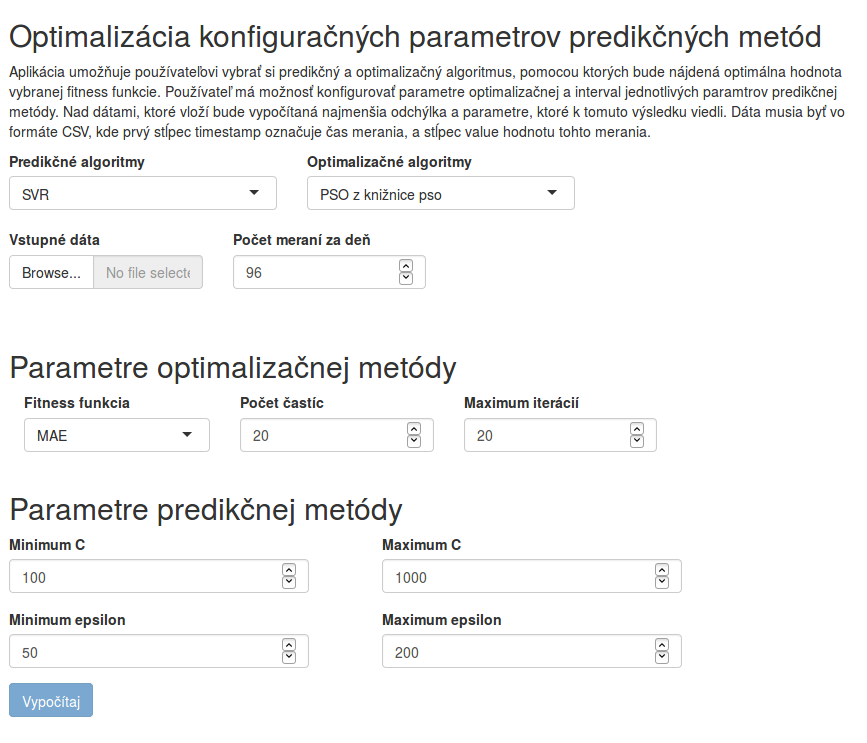
\includegraphics[width=\textwidth]{app_welcome.png}
  \caption{Úvodná obrazovka webovej aplikácie.}
  \label{fig-app-screen}
\end{figure}

\begin{figure}[H]
  \centering
  
\includegraphics[width=\textwidth]{app_data.png}
  \caption{Výber trénovacej a testovacej množiny.}
  \label{fig-app-data}
\end{figure}

Po vložení dát môže používateľ ďalej upravovať parametre, ktoré má k dispozícií.
Pri zmene prednastavených rozsahov pre dátové množiny netreba zabudnúť, že čím
bude väčšia testovacia množina dát, tým bude výsledná chyba menšia. Aplikácia
môže predpovedať dopredu jednu periódu alebo jej celé násobky. Zmena množiny,
z ktorej budú optimalizované parametre predikčnej metódy je priamo úmerná
času, ktorý bude zaberať výpočet. Rovnako pri navýšení hodnôt parametrov
optimalizačných metód ako je počet jedincov alebo iterácií, dochádza k získaniu
presnejšieho výsledku za cenu dlhšej odozvy. Toto samozrejme nemusí platiť vždy
a keďže používame algoritmy ako sú napr. náhodné lesy, vypočítaný výsledok môže
byť aj horší ako predchádzajúci. Nastavenie parametrov môžeme vidieť na
obrázkoch~\ref{fig-app-optimization} a~\ref{fig-app-prediction}.

\begin{figure}[H]
  \centering
  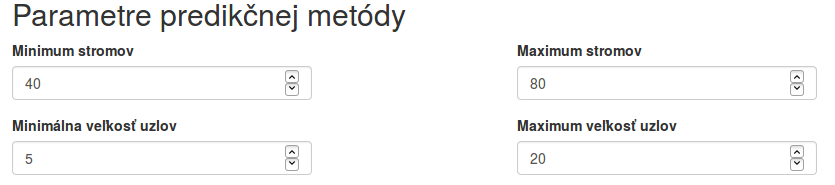
\includegraphics[width=\textwidth]{app_optimization.png}
  \caption{Výber parametrov optimalizačnej metódy.}
  \label{fig-app-optimization}
\end{figure}

\begin{figure}[H]
  \centering
  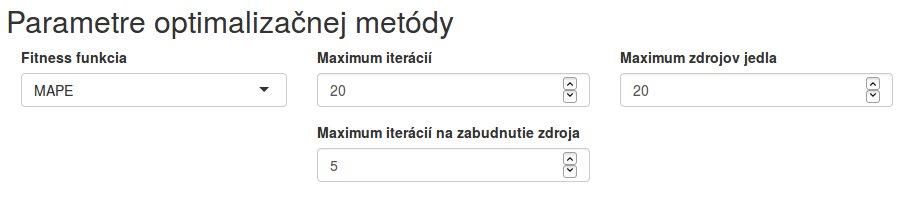
\includegraphics[width=\textwidth]{app_prediction.png}
  \caption{Výber paramterov predikčnej metódy.}
  \label{fig-app-prediction}
\end{figure}

Po kliknutí na tlačidlo ``Vypočítaj'' sa spustí výpočet a tlačidlo sa zakáže.
Povolené je v momente ukončenia výpočtu, kedy sa používateľovi zobraznia
výsledky. Výsledky pozostávajú z najmenšej chyby, ktorú zvolený algoritmus našiel,
tabuľku obsahujúcu parametre predikčnej metódy, ktoré viedli k tomuto výsledku
a graf zobrazujúci reálne a predpovedané hodnoty. Výstup aplikácie môžeme
vidieť na obrázku~\ref{fig-app-result}.

\begin{figure}[H]
  \centering
  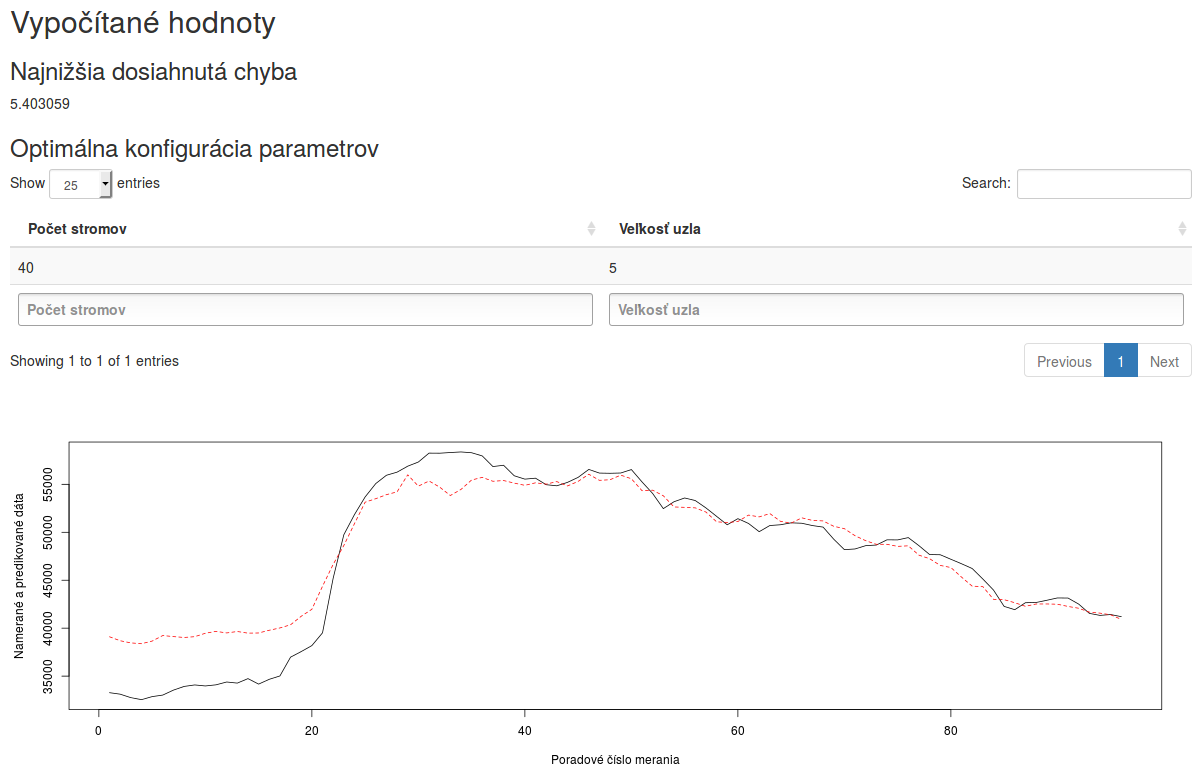
\includegraphics[width=\textwidth]{app_result.png}
  \caption{Zobrazenie vypočítaného výsledku používateľovi.}
  \label{fig-app-result}
\end{figure}

\newpage
\subsection{Obsah elektronického média}
\dirtree{%
  .1 CD nosič.
  .2 \textbf{doc}.
  .2 \textbf{conf}.
  .3 app-config.yml.
  .3 server-config.yml.
  .3 ui-config.yml.
  .2 \textbf{data}.
  .3 90\_UPLNE\_CONVERTED\_1W.csv.
  .3 90\_UPLNE\_CONVERTED.csv.
  .2 \textbf{src}.
  .3 00-read-data.R.
  .3 01-arima-prepare.R.
  .3 01-rf-prepare.R.
  .3 01-svr-prepare.R.
  .3 02-measure-error.R.
  .3 03-arima-predict.R.
  .3 03-rf-predict.R.
  .3 03-svr-predict.R.
  .3 04-abc-optimize.R.
  .3 04-pso-optimize.R.
  .3 04-psoptim-optimize.R.
  .2 \textbf{test}.
  .3 arima.R.
  .3 bf.R.
  .3 svr.R.
  .2 \textbf{web}.
  .3 bound-dates.R.
  .3 set-labels.R.
  .2 global.R.
  .2 server.R.
  .2 ui.R.
}

\begin{description}
  \item[$\bullet$ doc] dokumentácia, obrázky použité v nej a zdrojové súbory pre LaTeX
  \item[$\bullet$ conf] adresár obsahujúci konfiguračné súbory aplikácie
  \item[$\bullet$ data] vzorové vstupné dáta použité pri návrhu webovej aplikácie
  \item[$\bullet$ src] zdrojové súbory, v ktorých je implementovaná celá funkcionalita
  \item[$\bullet$ test] zdrojové súbry použité pri validácií riešenia
  \item[$\bullet$ web] zdrojové súbory pre Shiny
\end{description}

%-------------------------------------------------------------------------------
%   Appendix B - Future plans
%-------------------------------------------------------------------------------

\newpage
\section{Plán do letného semestra}

\begin{table}[H]
  \centering
  \begin{tabular}{||l|p{0.65\textwidth}||}
    \hline \hline
    \multicolumn{1}{|c|}{\textbf{\begin{tabular}[c]{@{}c@{}}Poradie týždňa \\ v letnom semestri\end{tabular}}} & \multicolumn{1}{c|}{\textbf{Popis plánovanej činnosti}}   \\ \hline
    \hline
    1. týždeň    &  úprava vstupných dát na požadovaný formát, aplikovanie predikčných algoritmov             \\ \hline
    2. týždeň    &  aplikovanie predikčných a optimalizačných algoritmov                                      \\ \hline
    3. týždeň    &  implementácia optimalizačných algoritmov, ktorým chýba podpora knižníc v jazyku R         \\ \hline
    4. týždeň    &  implementácia optimalizačných algoritmov, tvorba kostry grafického rozhrania aplikácie    \\ \hline
    5. týždeň    &  tvorba jednotného rozhrania medzi aplikáciou a grafickým rozhraním                        \\ \hline
    6. týždeň    &  implementácia grafického rozhrania a následne prepojenie s aplikáciou                     \\ \hline
    7. týždeň    &  ošetrenie neplatných akcií vykonané používateľom                                          \\ \hline
    8. týždeň    &  testovanie aplikácie na rôznych vstupných dátach používateľmi                             \\ \hline
    9. týždeň    &  tvorba technickej dokumentácie aplikácie                                                  \\ \hline
    10. týždeň   &  testovanie algoritmov, dokumentácia a porovnanie algoritmov                               \\ \hline
    11. týždeň   &  tvorba prezentácie a príprava na obhajobu projektu                                        \\ \hline
    \hline
  \end{tabular}
\end{table}

\end{document}

% Aplikácia je kvôli prehľadnosti organizovaná do viacerých adresárov. Pri
% vytváraní webovej aplikácie pomocou knižnice Shiny, sa program rozdeľuje na
% časť webového rozhrania a serverovú časť. Tie sa pri jednoduchých aplikáciách
% môžu nachádzať v jednom súbore, ja som ich podľa dokumentácie rozdelil do
% súboroc ``ui.R'' resp. ``server.R'' pre webové rozhranie resp. serverovú
% logiku. V adresári ``src''sa nachádzajú zdrojové súbory, ktoré v sebe zahŕňajú
% všetky výpočty aplikácie. Od prípravy vstupných dát, cez predikčné
% a optimalizačné algoritmy až po fitness funkcie. Adresár ``conf'' obsahuje
% konfiguračné súbory, ktoré poskytujú celej aplikácií flexibilitu pri jej
% ďalšom rozšírovaní a udržiavaní.

% \begin{table}[H]
%   \caption{Čo ešte určite musím stihnúť VYMAZAŤ (podľa dôležitosti)}
%   \centering
%   \begin{tabular}{|p{0.9\textwidth}|}
%     \hline
%     % pridať ACO od Marca Doriga      \\ \hline
%     % pridať regresné stromy          \\ \hline
%     % nájsť a pridať vzorec pre SVR   \\ \hline
%     pridať zhodnotenie analýzy      \\ \hline
%     pridať špecifikáciu požiadaviek (opis use case)   \\ \hline
%     % pridať exponencionálne vyrovnávanie               \\ \hline
%     % pridať učenie súborov klasifikátorov              \\ \hline
%   \end{tabular}
% \end{table}

% \paragraph{Autoregressive model}
% môže modelovať profil záťaže za predpokladu, že zátaž je lineárnou kombináciou
% predchádzajúcich záťaží\cite{KumarSingh2013}.

% \paragraph{Support Vector Machine based Techniques}
% je metóda analyzujúca dáta a rozpoznávajúca vzory, používaná na roztriedenie
% a regresnú analýzu, kombinuje zovšeobecnené riadenie
% s technikou ??????\cite{KumarSingh2013}.
%
% \paragraph{Support Vector Machine}
% je ML algoritmus používaný ako na klasifikáciu tak na regresiu
% support vector sú koordináty jednotlivých meraní napr. muž a žena a ich merané veličny reprezentované na osy, ktoré sú hraničnými elementami rôznych skupín
% maximalizuje rozmädzie medzi support vektormi jednej kategórie a support vektormi druhej kategórie, rozhodovacia funkcia je definovaná podmnožinou testovacej vzorky (jednotlivé supprot vektory)
% v 2D sú kategórie oddelené čiarou vo viacrozmerných dimenziách rovinou
%
% \paragraph{Incremental SVM}
% základom je pridávanie % http://www.jmlr.org/papers/volume7/laskov06a/laskov06a.pdf
% nový bod má najskôr pridelenú váhu 0, ak toto pridelenie nie je optimálnym riešením, teda bod sa môže stať support vectorom,
% váhy ostatných vektorov a rozhodovací prah musia byť aktualizované kvôli získaniu optimálneho riešenia nad novou množinou support vektorov
%
% \paragraph{Linear SVM}
% linárna kombinácia elementov (features, črty) značí, že sa jedná aj o lineárny klasifikátor  % http://stackoverflow.com/questions/6160495/support-vector-machines-a-simple-explanation
% napr ak (w1 * x1 + w2 * x2) > C potom element patrí do skupiny A, hodnotami x1 a x2 je element definovaný, tak ako je bod definovaný x a y súradnicou
% w je váha a C rozhodovacií prah, čiže ak nejaký ohodnotený element neprekročí hranicu spadá do jednej skupiny, ak prekročí spadá do druhej
%
% \paragraph{Concept drift}
% je správanie premennej, ktorú sa snažím predikovať sa môže časom meniť,
% čím sa postupne stáva model menej a menej presný\cite{Grmanova2016}.
%
% \paragraph{Online algorithm}
% spracováva vstup sériovo kúsok po kúsku, vstupné dáta nie sú dostupné na začiatku výpočtu % http://stackoverflow.com/questions/11496013/what-is-the-difference-between-an-on-line-and-off-line-algorithm
% musí spracovať vstup v jednej iterácií bez žiadnej podrobnej znalosti budúcich vstupov % https://xlinux.nist.gov/dads/HTML/online.html
% viac dát, časové obmedzenia, môže sa časom meniť % http://stats.stackexchange.com/questions/897/online-vs-offline-learning
%
% \paragraph{Offline algorithm}
% rieši problém od začiatku so všetkými vstupnými dátami % http://stackoverflow.com/questions/11496013/what-is-the-difference-between-an-on-line-and-off-line-algorithm
% vopred je daná celá séria vstupov % https://xlinux.nist.gov/dads/HTML/offline.html

% \paragraph{Kernel trick}
% problém nie je lineárne separovateľný, originálny nelineárny priestor % http://stats.stackexchange.com/questions/3947/help-me-understand-support-vector-machines
% je premietnutý do viacrozmerného priesotru pomocou nejakej nelineárnej transofrmácia s očakávaním, že to problém už bude riešiteľný
%
% \paragraph{Extreme learning machine}
% je novovznikajúca technika učenia poskytujúca efektívne % http://cherup.yonsei.ac.kr/files/Paper/2013_IEEE%20Intelligent%20Systems%20-%20Off%20line%20version_A%20System%20for%20Signature%20Verification%20Based%20on%20Horizontal%20and%20Vertical%20Components%20in%20Hand%20Gestures.pdf
% a zjednotené riešenie na všeobecné dopredné siete ako
% neurónové siete, RBF siete alebo kernelové učenie

% Časový rád je súbor meraní presne definovaných veličín získavaných opakovanými
% meraniami. Dáta zbierané zriedkavo alebo jednorázovo nepovažujeme za časový rád.
% Pozorované časové rády možno rozložiť na 3 zložky a to trendovú, sezónnu
% a nepravidelnú\cite{AustralianBureau}.

% Trendová zložka predstavuje smer veličiny v dlhodobom horizonte a máva klesajúci
% alebo stúpajúci charakter. Na druhej strane, sezónna zložka má cyklický
% charakter a dĺžka cyklu sa viaže napr. ku dňu, týždnu či roku. Nepravidelná
% zložka reprezentuje náhodné zmeny v prostredí, ktoré nie sú relevantné pre
% predpoveď časových rádov. Pri trénovaní modelu sa ich snažíme odfiltrovať
% optimálnou mierou natrénovania modelu.

% Pri predpovedaní časových radov ako napr. meraní odberu elektriky vznikajú 2 typy tvz. Concept drift.
% \textbf{Concept drift} je zmena správania veličiny, ktorú sa snažíme
% predpovedať. Model sa tak stáva postupne nepresný a je potrebné aby sa tejto
% zmene prispôsobil. Prvým typom je trvalá alebo dočasná zmena spôsobená
% ekonomickými alebo ekologickými faktormi. Druhým typom je sezónna zmena,
% spôsobená zmenami ročných období a množstvom denného svetla. Sezónnu zmenu
% môžeme pozorovať na úrovni dní, týždňov alebo rokov. Kvôli tomu je nutné
% v každom modely rozdeľovať tieto 2 typy concept drift\cite{Grmanova2016}.

% \subsection{Reziduálna zložka}
% Ostáva v časovom rade po odstránení trendovej, cyklickej a sezónnej zložky.
% Je tvorená náhodnými pohybmi v priebehu časového radu. Tiež pokrýva chyby
% v meraní. Obvykle sa predpokladá, že reziduálna zložka je biely šum, teda
% nekorelované náhodné veličny s nulovou strednou hodnotou\cite{http://www.math.sk/mpm/otazka_30.pdf}.

% ε-insensitive loss function defined
% \[
%     L_{\varepsilon}(y, f(x, w)) =
%     \begin{cases}
%       0 \text{ ak } |y - f(x, w)| \leq \varepsilon \\
%       |y - f(x, w)| - \varepsilon \text{ inak } \\
%     \end{cases}
% \]

% \begin{equation}
%   fitness = \delta + P
%   \label{eq-fitness}
% \end{equation}
% Faktor $\delta$ predstavuje rozdieľnosť výrazu aktuálneho chromozónu od
% cieľového chromozónu \cite{Simonova2007}

% \paragraph{Logistický regresný model}
% Nelineárna diskriminantná štatistická metóda. V \textbf{binary response} modely
% os $y$ zvyčajne reprezentuje individuálnu alebo experimentálnu jednotku. $Y$ môže
% nadobúdať hodnoty 0 alebo 1 pre situácie kedy udalosť nastane alebo nenastane.
% Os $x$ reprezentuje vysvetľujúcu veličinu ako vektor, ktorý môže znázorňovať
% pravdepodobnosť udalosti $(Y = 1)$~\cite{Li2010}.

%-------------------------------------------------------------------------------
%   Naive methods
%-------------------------------------------------------------------------------

% \subsubsection{Naivné metódy}
% Predpovede sú vytvárané pomocou posledných hodnôt alebo ich priemerov.
%
% \paragraph{Seasonal naïve method}
% Poslednú nameranú hodnotu použijeme ako predpoveď pre nasledujúce obdobie. Ak
% sú naše dáta vysoko závisle od ročného obdobia, je lepšie použiť na predpoveď
% hodnotu z rovnakého obdobia, napr. z minulého roka~\cite{Grmanova2016}.
%
% \paragraph{Naïve average long-term method}
% Predpokladá, že dáta obsahujú vzory, ktoré nie sú závislé od ročných období.
% Kvôli tomu sú časové rady lokálne stabilné s pomaly meniacim sa priemerom.
% Hodnotu, ktorú použijeme ako predpoveď je iba priemorom viacerých posledných
% hodnôt~\cite{Grmanova2016}.
%
% \paragraph{Naïve In median long-term method}
% Táto metóda je alternativou k predchádzajúcej metóde. Keďže priemerom nedokáže
% model dostatočne rýchlo reagovať na rapídne výkyvy a abnormality, lepšie
% výsledky dosiahneme nahradením priemeru za median posledných \textit{n}
% meraní~\cite{Grmanova2016}.

% Predpovedanie veličín, ktoré My sme sa zamerali na predpovedanie veličín , ktorých predpoveď môže závisieť od
% iných veličín, ale
%
% V práci sme sa zamerali na p Predpovedanie sa tak stáva  čo či tý Väčšiu spotrebu elektrickej energie máme počas práce či
%
% zábave, naopak len minimum spotrebujeme počas spánku. Už len z tohto príkladu
% je zrejmé, spotreba elektriny ľudí sa líši od ich správania, zvyklostí či
% možností, ale aj faktorov, ktoré pôsobia na nás všetkých ako je počasie, deň
% v týždni, pracovné voľná či kultúrne tradície. Faktom je, že spotreba elektriky
% bude naďalej rásť, keďže celý svet postupne minimalizuje závislosť na
% neobnoviteľných zdrojoch energie a náhradou má byť práve elektrická energia.
%
% Pre efektívnu výrobu a distribúciu elektriky je potrebné vedieť predpovedať
% jej spotrebu, čím zamedzíme ekonomickým stratám ako na strane výrobcu tak aj na
% strane spotrebiteľa. Predpoveď by sa, v ideálnom prípade, mala líšiť od
% skutočnej hodnoty minimálne a

% V literatúre označovaný ako ABC algoritmus (Artifical bee colony) je pomerne
% nový medzi rojovými algoritmami. Princíp je založený na biologickom procese,
% správaní medonosných včiel pri hľadaní potravy. Hlavný mechanizmus ktorým včely
% optimalizujú množstvo procesov je tzv. včelí tanec (\textbf{waggle dance}),
% ktorým včely lokalizujú zdroje potravy a nachádzajú ďalšie~\cite{Chavan2015}.
%
% Každá včela na pracujúca v roji sa spolupodiela na tvorbe celého systému na
% globálnej úrovni. Správanie systému je určené lokálnym správaním, kde spolupráca
% a zladenie jedincov vedie k štruktúrovanému kolaboračnému systému~\cite{Chavan2015}.
%
% Algoritmus funguje na princípe, že včely nájdu najviac výnosný zdroj
% s použitím, čo najmenšej energie. \textbf{Foragers} (zrejme robotnice hľadajúce zdroj jedla) uvažujú
% presúvanie sa medzi zdrojmi nektárov na základe kvality alebo zisku zdroju.
% Algoritmus poskytuje samo-manažovateľné a samo-organizované riešenie, vo svojej
% podstate decentralizované, pre daný problém~\cite{Buhussain2016}.

% %-------------------------------------------------------------------------------
% %   Ensemble learning
% %-------------------------------------------------------------------------------
%
% \subsubsection{Učenie súborov klasifikátorov}
% Používa sa na jednodňovú predikciu. Ak \textit{h} je počet meraní, ktoré sú
% denne dostupné, v deň \textit{t} sa vykoná \textit{h} predikcií podľa váženého
% priemeru \textit{m} modelmi. Nasledujúci deň sa vypočíta chyba predpovede,
% na základe ktorej sa znova prepočítajú váhy a každý model sa
% aktualizuje\cite{Grmanova2016}.
%
% Učenie súborov klasifikátorov môžeme rozdeliť na homogénne a heterogénne učenie.
%
% \paragraph{Homogénne učenie súborov klasifikátorov}
% Pozostáva z modelov rovnakého typu, ktoré sa učia na rôznych podmnožinách
% datasetu.
% \paragraph{Heterogénne učenie súborov klasifikátorov}
% Aplikuje rôzne typy modelov nad rovnakými dátovými množinami\cite{Grmanova2016}.
%
% %-------------------------------------------------------------------------------
% %   Exponential smoothing
% %-------------------------------------------------------------------------------
%
% \subsubsection{Exponencionálne vyrovnávanie}
%
% Táto metóda, tak ako vyššie popísané metódy, najprv na základe dát
% z predchádzajúcich meraní vytvorí model. Ten sa v ďalej použíje na
% redpovedanie budúcich dát. Tento vzťah môžeme matematicky zapísať ako
% \begin{equation}
%   y(t) = \beta(t)^T f(t) + \varepsilon(t)
%   \label{eq-expo}
% \end{equation}
% Vo vzorci \ref{eq-expo} sa opäť nachádza biely šum $\varepsilon(t)$. Hodnota
% $\beta(t)$ predstavuje \textbf{coefficient vector} a $f(t)$
% \textbf{fitting function}~\cite{Mahalakshmi2016}.
%
% Jednou z predikčných metód časových radov, ktorá používa exponencionálne
% vyrovnávanie je aj Wintersova metóda. Pri sezónnych dátach sú použité 3
% vyrovnávacie parametre a to trend, sezónosť a stacionárnosť. Analýza
% a predpoveď priamym aplikovaním Wintersovej metódy môže byť náročné, keďže
% dátové množiny väčšinou obsahujú \textbf{riedke pozorovania (sparse values)}.
% Tento problém môžeme vyriešiť kombináciou ostatných metód, ako je napr.
% autoregresívny model či spektrálna analýza, s exponencionálnym
% vyrovnávaním~\cite{Mahalakshmi2016}.

% %-------------------------------------------------------------------------------
% %   Ant colony optimization
% %-------------------------------------------------------------------------------
%
% \subsubsection{Kolónia mravcov}
% Pri tomto algoritme, mravce tiež opúšťajú mravenisko, kvôli hľadaniu zdrojov
% potravy náhodne. Potom vyhodnotia kvalitu zdroja potravy a donesú ho naspäť do
% mraveniska. Zanechávajú pri tom na zemi chemické stopy. Sila týchto stôp závisí
% od kvality nájdeného zdroja potravy. Mnoho výskumov využíva tento algoritmus na
% riešenie NP problémov, ako napríklad problém obchodných cestujúcich,
% vyfarbovanie grafov, smerovnaie áut alebo plánovacie problémy. Používa sa aj pri
% \textbf{cloud computing} na nájdenie optimálneho riešenia pri plánovaní úloh
% pre virtuálne servery~\cite{Buhussain2016}.
%
% Keď mravce hľadajú potravu prvý krát, hľadajú náhodne až kým nenájdu zdroj
% potravy. Zanechávajú pri tom za sebou chemickú stopu nazývanú feromón, ktorá
% tak vedie k zdroju. Tá následne priťahuje ostatné mravce k tomuto zdroju
% potravy. Tento proces pokračuje pokiaľ mravce nenájdu najkratšiu cestu vedúcu
% ku konkrétnemu zdroju potravy. Najkratšia cesta je určená naakumulovaným
% množstvom feromónov na ceste k zdroju potravy~\cite{Buhussain2016}.

%-------------------------------------------------------------------------------
%   Chapter X - Conclusion
%-------------------------------------------------------------------------------

% \chapter{Záver}
% Tu bude záver

% Kapitola \chapter{Nazov}
% Necislovana kapitola \chapter*{Nazov}% underline \underline{science}
% Pokapitola (Section) \section{Nazov}
% Subsection \subsection{Nazov}
% Paragraph \paragraph{Nazov}
% Ak niečo nechceme číslovať, použijeme *, avšak, ak to chceme v obsahu, musíme to do neho pridať

% \Huge, \huge, \LARGE, \Large, \large, \normalsize, \small, \footnotesize, \tiny
% italic \textit{accident}.
% bold \textbf{greatest}
% -1 part     1 section     3 subsubsection  5 subparagraph
%  0 chapter  2 subsection  4 paragraph
